% Template for package SVJour3
% Springer journals, Heidelberg, 2010/09/16

\RequirePackage{fix-cm}
\documentclass{svjour3}
% onecolumn (standard format)
%\documentclass[smallcondensed]{svjour3}
% onecolumn (ditto)
%\documentclass[smallextended]{svjour3}
% onecolumn (second format)
%\documentclass[twocolumn]{svjour3}
% twocolumn
\smartqed  % flush right qed marks to end of proof
%\usepackage{amsbsy}
%, amsmath,amsfonts,amsthm,amscd,amssymb,latexsym}
\usepackage{graphicx}

\usepackage{mathspec}
\usepackage{float}
% use Times fonts if available on your TeX system
% \usepackage{mathptmx}
\usepackage{latexsym}

\usepackage{caption}
\usepackage{subcaption}
%\usepackage{svg}
% definitions here
% \newcommand{}{}
%\theoremstyle{definition}
\usepackage{color,enumitem,graphicx}
 

\newtheorem{observation}{Observation}
%\newtheorem{lemma}[theorem]{Lemma}
%\newtheorem{corollary}[theorem]{Corollary}

\usepackage{hyperref}
 
\journalname{The Mathematical Intelligencer}
%
\begin{document}

\title{Can the Elliptic Billiard Still Suprise Us?}

\author{Dan Reznik \and Ronaldo Garcia \and Jair Koiller}

\authorrunning{Reznik, Garcia and Koiller}

\institute{D. Reznik \at Upper West Soluções \email{dreznik@gmail.com} \and
R. Garcia \at Universidade Federal de Goiás \email{ragarcia@ufg.br} \and 
J. Koiller \at Universidade Federal de Juiz de Fora \email{jairkoiller@gmail.com}}

\date{Received: date / Accepted: date}

\maketitle

\begin{abstract}
Experimentation with closed trajectories in Elliptic Billiards reveals, for the $N=3$ family, surprising new loci invariants. These have been subsequently proven and generalized $\forall{N}$.

\keywords{elliptic billiard, triangular orbits, elliptic loci}

\noindent \textbf{MSC} {51M04 \and 37D50  \and 51N20\and 51N35\and 	68T20}
\end{abstract}

\section{Introduction}
\label{intro}
\begin{quote}
Things in motion sooner catch the eye\\
Than what not stirs. --W.S., ``Troilus and Cressida'' 
\end{quote}

Old objects will sometime reveal new secrets when put in motion. In 2011 we uploaded a video \cite{dsr_vid11d} showing the family of 3-periodic {\em orbits} in an Elliptic Billiard  \cite{sergei91,birkhoff66}. We drew the locus of the {\em Incenter} and intouch points \cite{mw}. The former describes an ellipse while the latter is more complex, with two internal self-intersecting lobes, Figure~\ref{fig:intro-plot}.

\begin{figure}
    \centering
    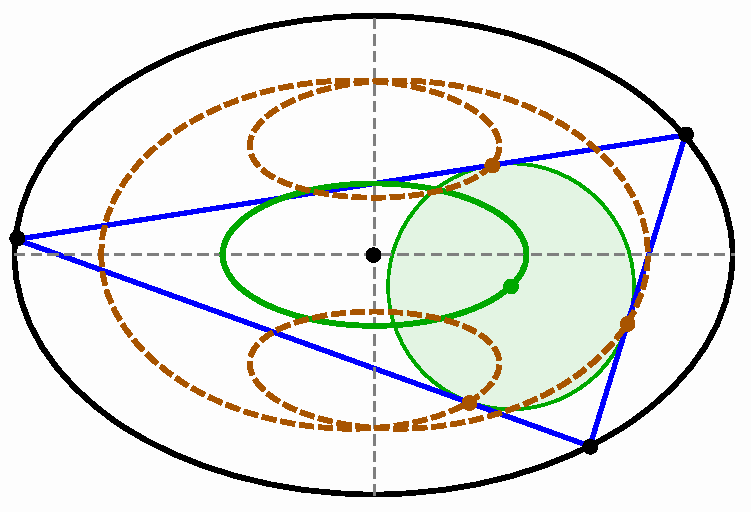
\includegraphics[width=.5\textwidth]{pics/0001_intro_plot.pdf}
    \caption{An $N=3$ orbit (blue), its Incircle (transparent green), Incenter (green dot) and contact points (brown dots) are shown. Over the $N=3$ family, the Incenter locus is an ellipse (green), and that of the intouch points is a self-intersecting curve with two internal lobes (dashed brown).}
    \label{fig:intro-plot}
\end{figure}

Over the next few years there surfaced elegant proofs for the ellipticity of the Incenter \cite{olga14,ronaldo16} as well as for that of the Barycenter \cite{sergei2016,ronaldo19}, Circumcenter  \cite{corentin19,ronaldo19}, and Orthocenter \cite{ronaldo19}.

Here we describe a second exploratory cycle, some eight years after our original video. As before, we began with loci of Triangular Centers \cite{mw}. The curves we obtained went from expected, to new, to amazing: elliptic, non-elliptic, quasi-elliptic, with kinks, similar or identical to the Billiard (or its Caustic), point-like, and even perfectly circular!

Beyond loci, $N=3$ revealed an amazing property: the ratio of Inradius to Circumradius is invariant, and this implies beautiful relations involving orbit angles and areas.
Here,  invariant means that the property is shared for all 3-periodic orbits of the billiard. Other suprising invariants were that the $N=3$ family has a stationary Mittenpunkt \cite{mw} and a stationary Cosine Circle \cite{mw}. 

Close observation of the $N=4$ family, closely related to Monge's Orthoptic Circle \cite{connes07}, Figure~\ref{fig:monge-orthoptic}, provided us clues with which to generalize all $N=3$ thus found for all $N$, namely the fact that these two (i) contain a stationary point, (ii) a stationary circle, and (iii) preserve angular and area relations. These investigations are summarized in Figure~\ref{fig:global-diagram}.

\begin{figure}[H]
    \centering
    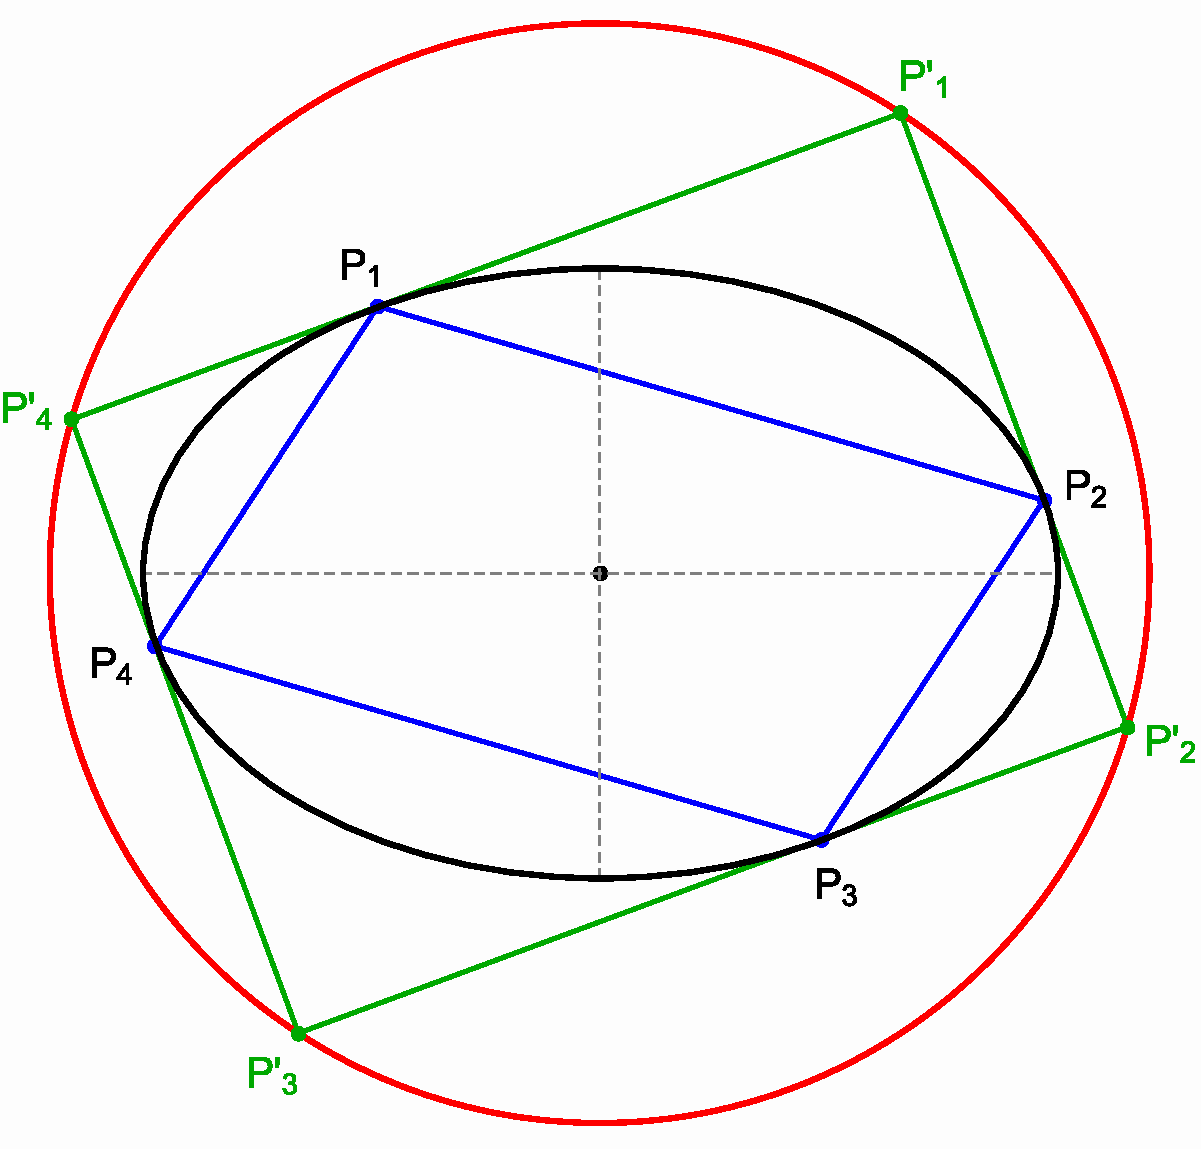
\includegraphics[width=.4\textwidth]{pics/0200_monge_orthoptic.pdf}
    \caption{French Mathematician Gaspard Monge (1746-1818) discovered that the locus of points whose tangents to a given ellipse subtend a right angle is a circle (red). Here's the connection to Billiards: take a point $P_1'$ on Monge's Circle and extend one tangent till it hits the circle again $P_2'$. Repeat this twice so as to yield four vertices on the circle. Suprisingly, these form a rectangle, and its four points of tangency $P_1P_2P_3P_4$ define an inscribed parallelogram  which is a billiard orbit of the ellipse! Note: the family of $N=4$ billiard orbits are constant-perimeter parallelograms.}
    \label{fig:monge-orthoptic}
\end{figure}

\begin{figure}[H]
    \centering
    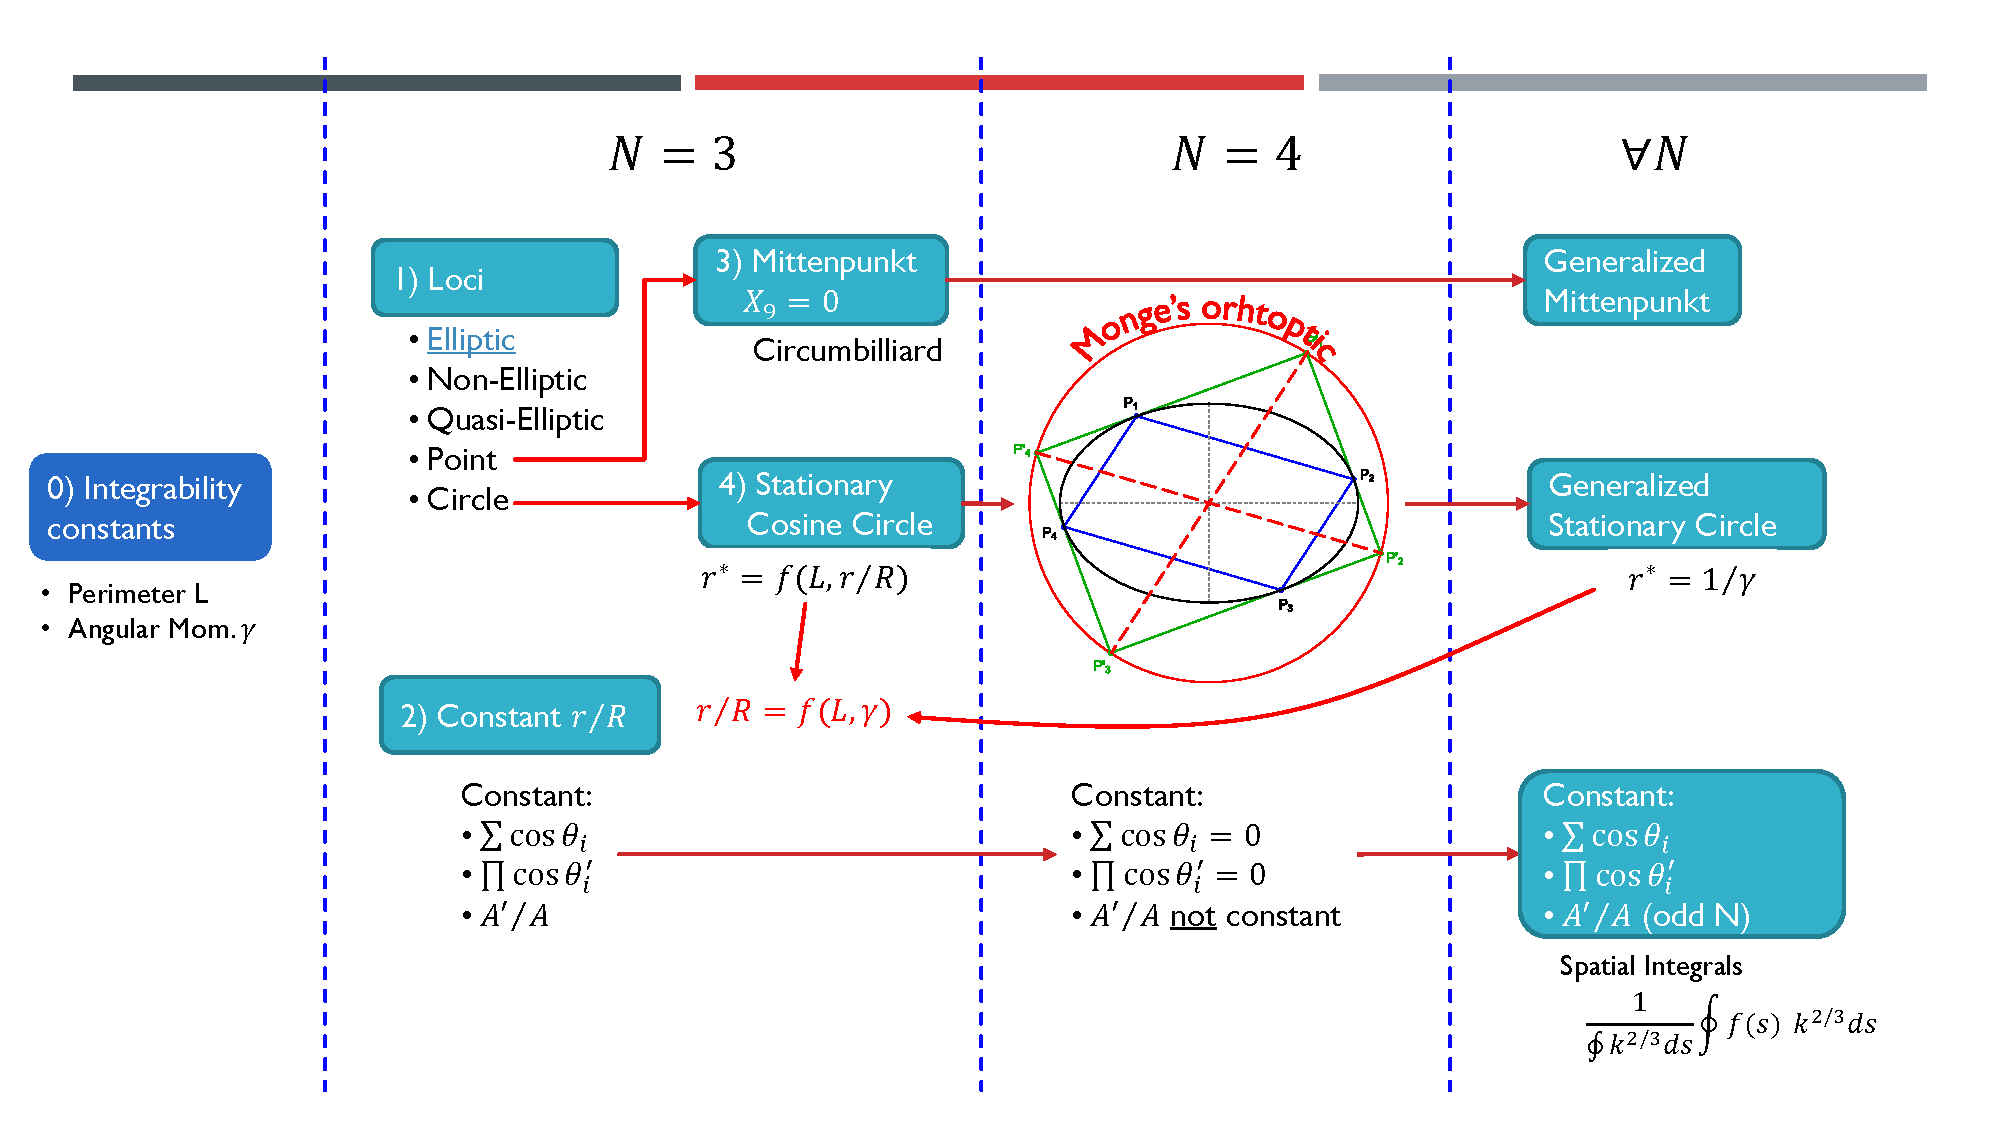
\includegraphics[width=\textwidth]{pics/0002_diagram_slide.pdf}
    \caption{A bird's eye view of our exploration. From left to right: (i) we start with know results from the integrability of the Elliptic Billiard, namely constant orbit perimeter $L$ and constant Joachmisthal's angular momentum $\gamma$. We then (ii) investigate various properties of the $N=3$ family. (iii) Close observation of the $N=4$ family provides clues to (iv) generalizations of all propertiees $\forall{N}$. A key unification (red arrows) is expressing $r/R$ in terms of $S$ and $\gamma$.}
    \label{fig:global-diagram}
\end{figure}

In the remainder of this paper we will describe our explorations in the following order:

\begin{itemize}
    \item Beautiful elliptic and non-elliptic loci.
    \item The Mittenpunkt: a point-like locus.
    \item The $r/R$ invariant and its corollaries.
    \item The Cosine Circle: a circular locus.
    \item Generalizing all results to $N>3$.
\end{itemize}

Many of our key observations are available as online videos, images, and applets \cite{reznik_media}. We also maintain a companion website \cite{reznik_web} where details about this work are constantly added and/or updated.

\section{Kinemagic Loci}
\label{sec:loci}
\subsection{Incenter Locus Recap}

Consider an Elliptic Billiard \cite{sergei91} centered at $O$, and an $N=3$ periodic trajectory $P_1P_2P_3$, called an {\em orbit}, shown in Figure~\ref{fig:single-orbit}. A vertex bisector is congruent with inward normal to the Ellipse, and these meet at the Incenter $X_1$ \cite{etc}.\\

\noindent Note: Triangular centers (such as the Incenter, Barycenter, etc.) will be referred here by their Kimberling Codes \cite{etc}: $X_1$ for the Incenter, $X_2$ for the Barycenter, etc. Also, $a$ refers to the the Billiard's axis ratio and when not specified, $a=1.5$.

\begin{figure}[H]
     \centering
     \begin{subfigure}[t]{0.45\textwidth}
         \centering
         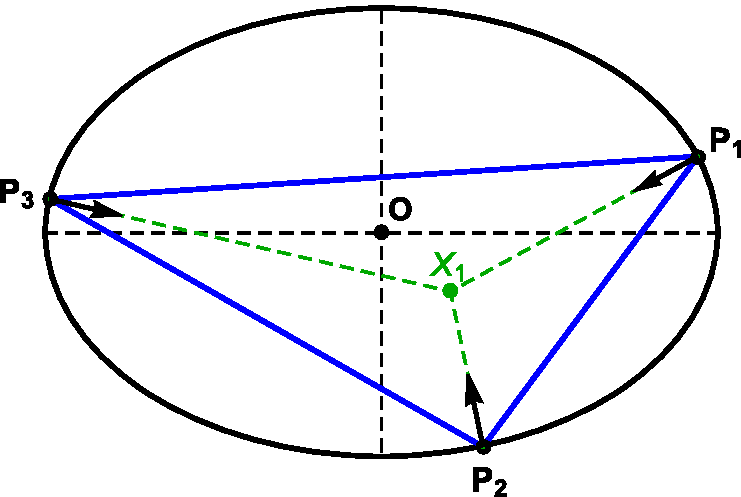
\includegraphics[height=.65 \linewidth]{pics/0000_single_orbit.pdf}
         \caption{An $N=3$ periodic trajectory, called an {\em orbit}, and its Incenter $X_1$: where the bisectors concur.}
         \label{fig:single-orbit}
     \end{subfigure}
     \hfill
     \begin{subfigure}[t]{0.45\textwidth}
         \centering
          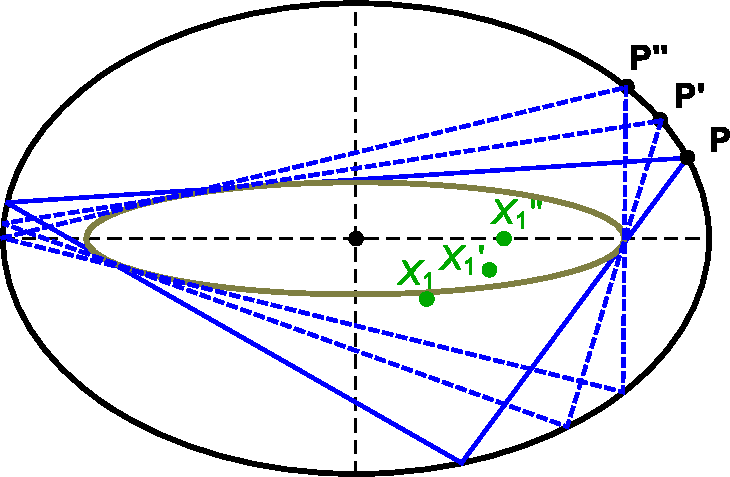
\includegraphics[height=.65\linewidth]{pics/0010_three_orbits.pdf}
         \caption{Three triangular orbits, each associated with a {\em leader} vertex $P,P',P''$, and their Incenters $X_1,X_1',X_1''$, and the confocal Caustic.}
         \label{fig:three-orbits}
     \end{subfigure}
     \caption{Triangular Orbits in an Elliptic Billiard and their Incenter.}
\end{figure}

Poncelet's Porism \cite{dragovic11} states that if one $N$-periodic trajectory can be found starting at a point $P$ on the boundary, then every boundary point can also initiate an $N$-trajectory, i.e., there exists a one-dimensional {\em family} of orbits.

The ellipse is the only planar Billiard with an Integrable Hamiltonian \cite{birkhoff66}. A well-known corollary is that all orbits will have fixed perimeter $L$. For $N=3$ we have derived its expression with respect to the Billiard's aspect ratio: \cite{ronaldo19a}:

\begin{eqnarray}
L&=&\frac{2(\delta+a^2+1)\sqrt{2\delta-a^2-1}}{a^2-1}\\
\delta&=&\sqrt{a^4-a^2+1}
\end{eqnarray}

Joachimsthal's Integral  \cite{sergei91} states that a positive quantity $\gamma$, called the {\em angular momentum} is conserved. This is the scalar product of velocity with the gradient at any orbit vertex:

\begin{equation}
 \gamma=\hat{v}.\nabla{f}(P)=\mbox{constant},\forall{P}
 \label{eqn:joachim}
\end{equation}

\noindent where $P$ is a vertex of the orbit, $\hat{v}$ is the incoming orbit edge, and:

\begin{equation}
f=\frac{1}{2}\left(\frac{x^2}{a^2}+\frac{y^2}{b^2}\right)
\label{eqn:f}
\end{equation}

Geometrically, constant $\gamma$ is equivalent to stating all trajectory edges are tangent to a confocal ellipse, called the {\em Caustic}, Figure~\ref{fig:three-orbits}. For $N=3$ we can express it in terms of the Billiard aspect ratio:

\begin{equation}
\gamma = \frac{\sqrt{2\delta-a^2-1}}{a^2-1}
\label{eqn:gamma}
\end{equation}


Consider the three $N=3$ orbits in Figure~\ref{fig:three-orbits}, identified by a starting vertex $P,P',P''$, called the {\em leader}, as well as their Incenters $X_1,X_1',X_1''$. Let the leader be parametrized continuously:

\begin{equation}
P_1(t)=\left(a\cos{t},\sin{t}\right),\,t\in\left[0,2\pi\right)
\label{eqn:tparam}
\end{equation}

In \cite{ronaldo19} we are provided explicit equations for $P_2$ and $P_3$ in terms of $P_1$, and the dependence is highly non-linear. Though the Incenter's trilinear coordinates \cite{mw} are of the simplest form, $1:1:1$ \cite{etc}, its Cartesian location will be non-trivial given $P_2,P_3$ non-linearities. This renders remarkable the following theorem, which we borrow from \cite{olga14}: 

\begin{theorem}
The locus of the Incenter is elliptic.
\end{theorem}

Also elliptic are the loci of the Barycenter $X_2$, the Circumcenter $X_3$, the Orthocenter $X_4$, and the 9-Point Circle Center $X_5$ \cite{sergei2016,corentin19,ronaldo19}, Figure~\ref{fig:locus-x12345}. These can be viewed as an animation \cite[video \#1]{dsr_main_videos_2019} and interactively \cite{dsr_applet_x12345}.

\begin{figure}[H]
     \centering
     \begin{subfigure}[m]{0.45\textwidth}
     \centering
     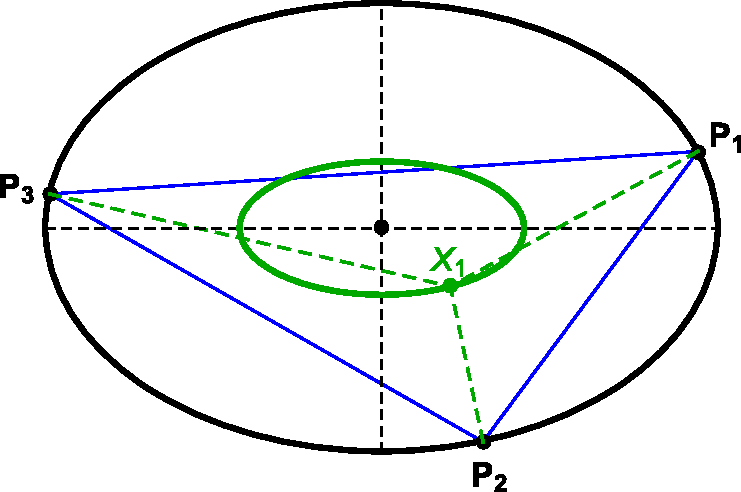
\includegraphics[height=.65\linewidth]{pics/0020_incenter_locus.pdf}
         \caption{The elliptic locus of the Incenter $X_1$.}
        \label{fig:locus-incenter}
     \end{subfigure}
     \hfill
     \begin{subfigure}[m]{0.45\textwidth}
         \centering
         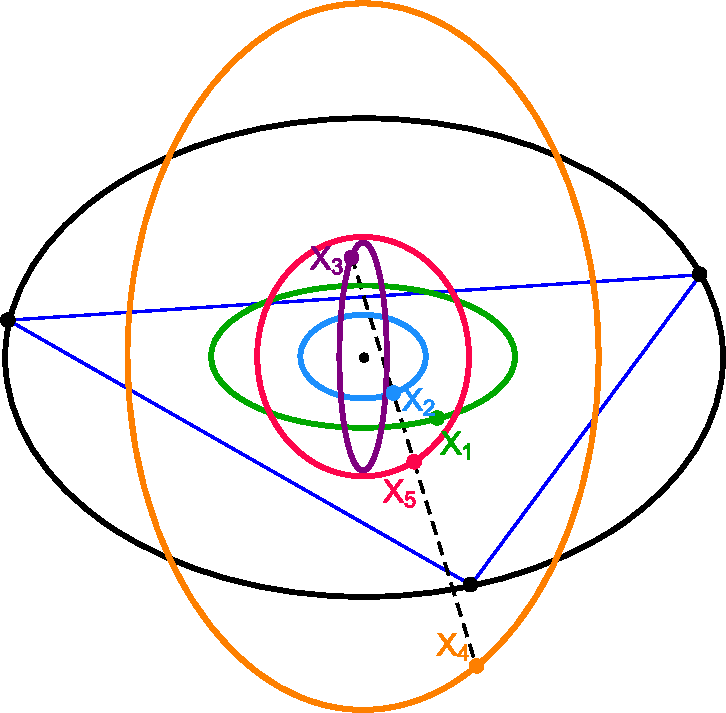
\includegraphics[height=\linewidth]{pics/0030_x12345_locus.pdf}
         \caption{Elliptic Loci of Incenter $X_1$, Barycenter $X_2$, Circumcenter $X_3$, Orthocenter $X_4$, and Center of the 9-Point Circle $X_5$.}
         \label{fig:locus-x12345}
     \end{subfigure}
     \caption{Elliptic Loci of major triangular centers.}
\end{figure}

\subsection{Eccentric Excenters}

Closely related to the Incenter are the {\em Excenters} \cite{mw}, the three meetpoints of perpendiculars to bisectors and vertices of the Excentral Triangle \cite{mw}. It turns out their locus is also elliptic and similar to a rotated version of the Incenter's  \cite{ronaldo19}, Figure~\ref{fig:locus-incenter-excenter}.
%

\begin{figure}[H]
    \centering
    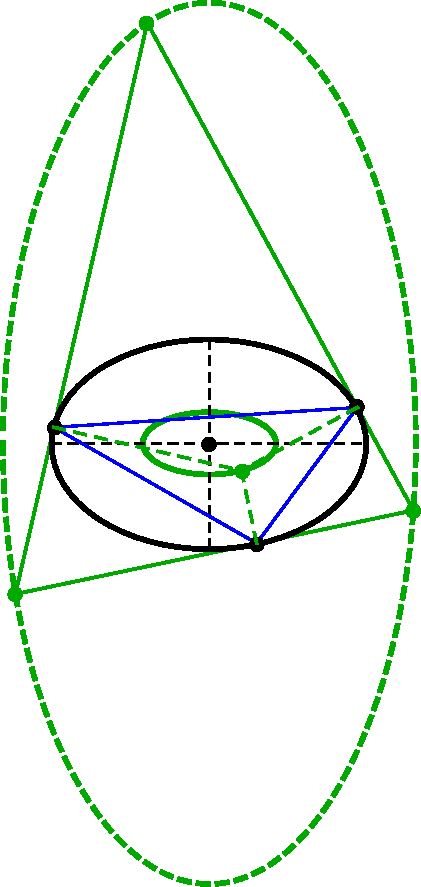
\includegraphics[angle=90,width=.73\textwidth]{pics/0025_incenter_excenter_locus.pdf}
    \caption{A Billiard is shown in black with its axes rotated (to save space), as well as an $N=3$ orbit (blue) and its Excentral Triangle (solid green). The vertices of the Excentral Triangle move along an elliptic locus similar to a perpendicular copy of the Incentral locus (shown solid green inside the Billiard).}
    \label{fig:locus-incenter-excenter}
\end{figure}

Though the vertices of the Excentral Triangle sweep an ellipse, consider those of the {\em Intouch Triangle}, formed by the three points of contact of the Incircle with the orbit. As shown in an early video \cite{dsr_vid11b}, their locus is self-intersecting with two lobes.

Generally, the locus of vertices of an orbit's derived triangle Figure~\ref{fig:derived-tris} are non-elliptic. Besides the Intouch vertices, those of the Feuerbach, and Medial Triangles \cite{mw} sweep non-elliptic curves. Surprisingly, the vertices of the {\em Extouch Triangle}, where Excircles touch the orbit sides, are not-only elliptic, but congruent with the Caustic! This is shown on Figure~\ref{fig:non-elliptic}.



\begin{figure}[H]
    \centering
    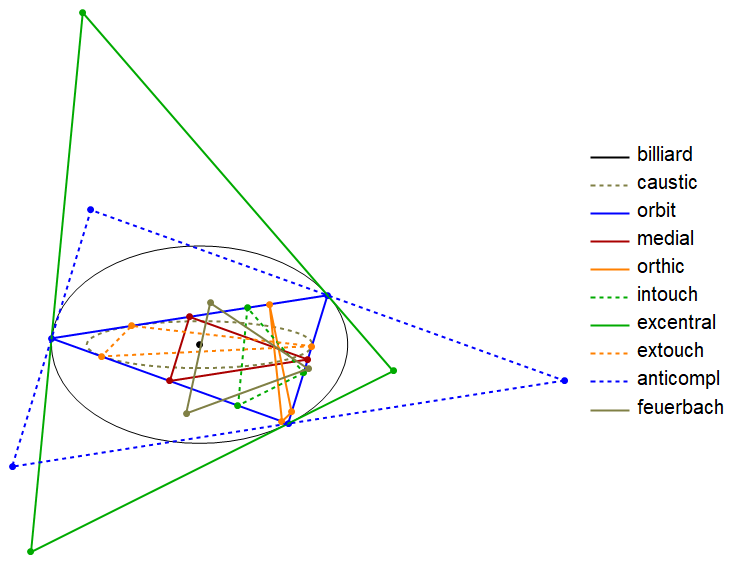
\includegraphics[width=.75\textwidth]{pics/0043_derived-triangles.png}
    \caption{A billiard is shown (black as well as an orbit (blue) and its Caustic (dashed brown). Several triangles derived from the orbit are shown, and indicated on the legend.}
    \label{fig:derived-tris}
\end{figure}
%
\begin{figure}[H]
    \centering
    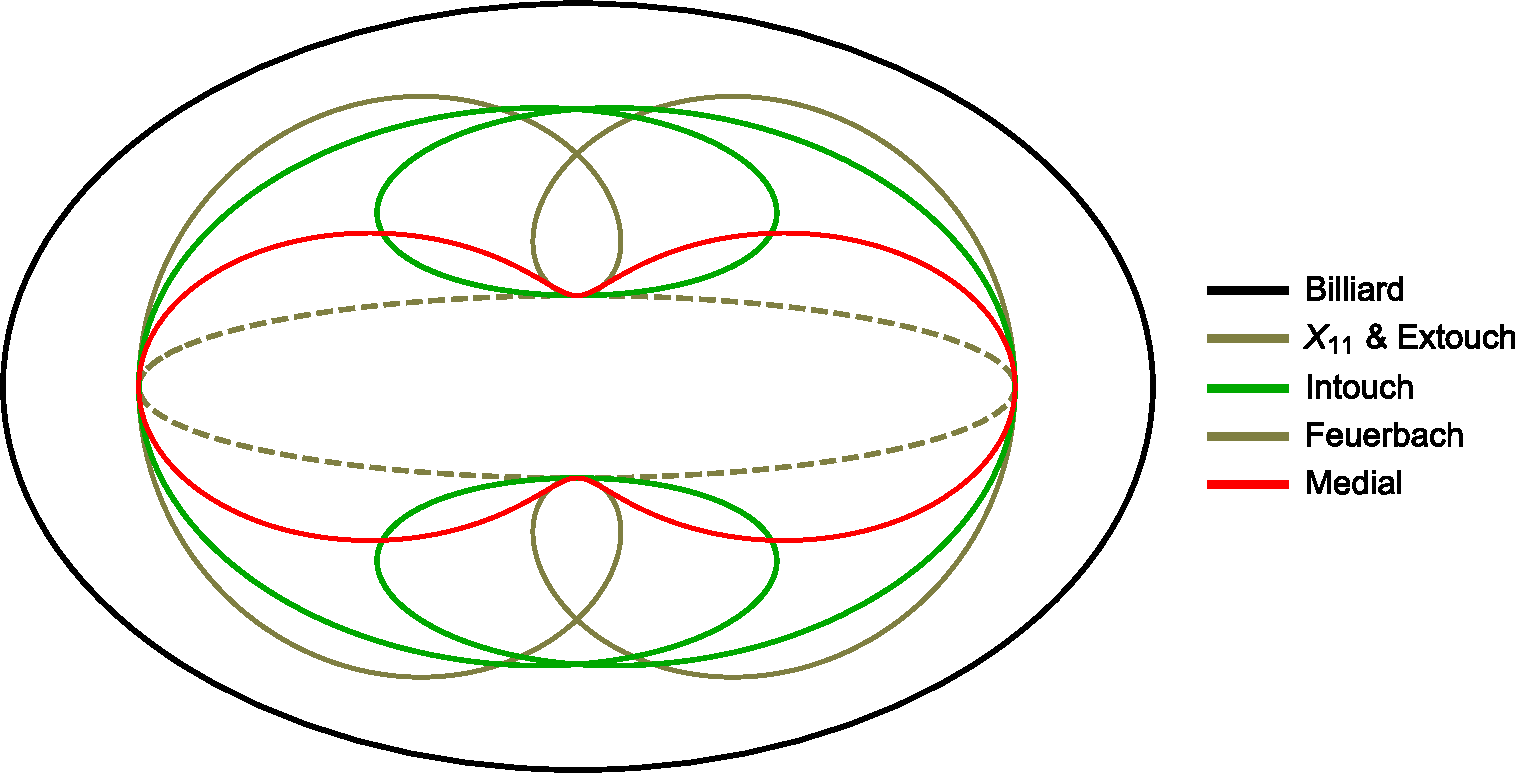
\includegraphics[height=.35\linewidth]{pics/0040_non_elliptic.pdf}
    \caption{The vertices of the Intouch (green), Feuerbach (brown), and Medial (red) Triangles sweep non-elliptic loci. Surprisingly, the extouch points (as well as the Feuerbach Point $X_{11}$, sweep the Caustic.}
    \label{fig:non-elliptic}
\end{figure}
The causes for ellipticity vs. non-ellipticity of loci of vertices of derived triangles is not   understood.
\subsection{Fiery Feuerbach}

The Feuerbach Point $X_{11}$ is the single point of contact between the Incircle and the 9-Point Circle \cite{mw}. Remarkably, and just like the vertices of the Extouch Triangle, its locus is also congruent with the $N=3$ Caustic Figure~\ref{fig:feuer_loci}.

Interestingly, if orbit vertices slide along the Billiard in one direction, $X_{11}$ (resp. the Extouch Points) will sweep the Caustic in the opposite (resp. same) direction \cite[video \#2]{dsr_main_videos_2019}.
%
\begin{figure}[H]
    \centering
    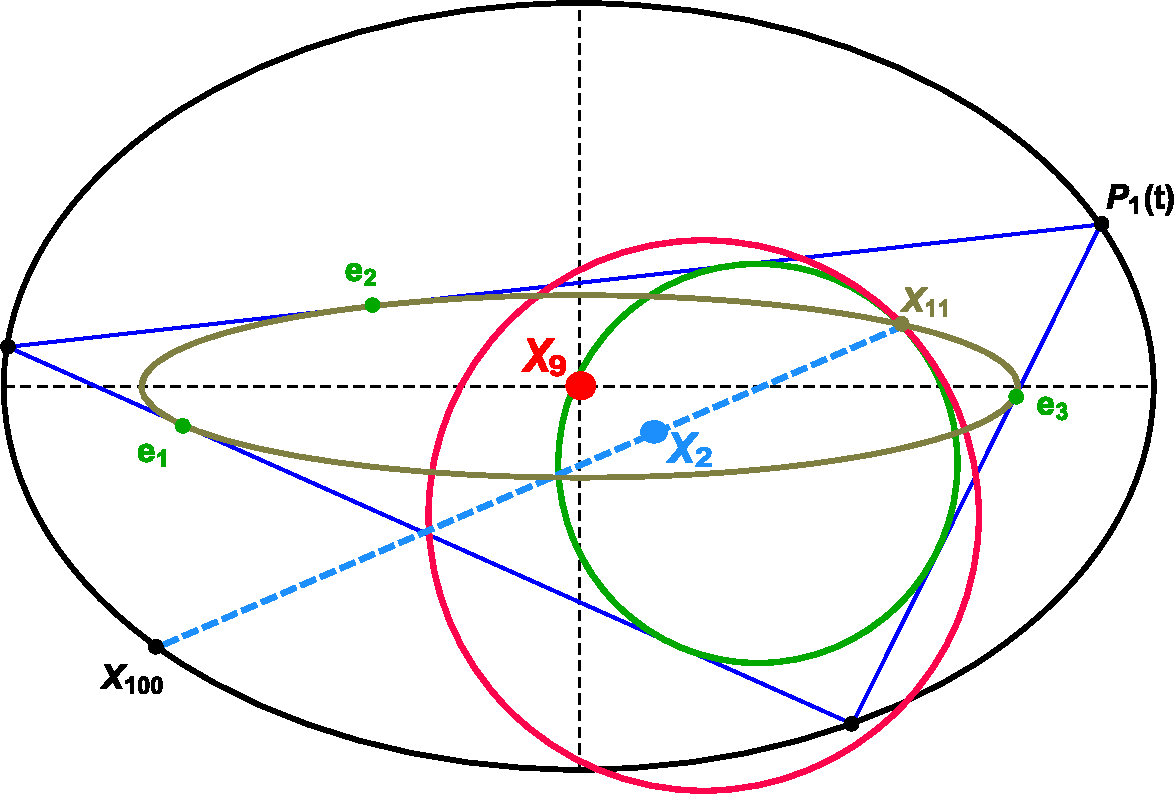
\includegraphics[width=.60\textwidth]{pics/0035_feuerbach_loci.pdf}
    \caption{Shown is the Elliptic Billiard (black), as well as an $N=3$ orbit (blue), with $P_1(t)$ the leader vertex, and the Caustic (brown). Also shown are the orbit's Incircle (green) and 9-Point Circle (pink), whose single point of contact is the Feuerbach Point $X_{11}$. Shown also is its anticomplement $X_{100}$, and the three Extouch Points $e_1,e_2,e_3$. Remarkable properties include: $X_{11}$ and the extouch points sweep the Caustic, and $X_{100}$ sweeps the Billiard (in opposite directions).}
    \label{fig:feuer_loci}
\end{figure}

Just as remarkably, $X_{100}$, the {\em anti-complement} \cite{mw} of the $X_{11}$, i.e., the latter's double-length reflection about the Barycenter $X_2$, is congruent with the Billiard \cite[video \#4]{dsr_main_videos_2019}. Also congruent with the Billiard, though not understood, is the locus of $X_{88}$.

\begin{observation}
The locus of $X_{11}$, the Feuerbach Point, is congruent with the $N=3$ Caustic and the locus of $X_{100}$, the anti-complement of the Feuerbach Point, is congruent with the Billiard, as is that of $X_{88}$.
\end{observation}

\subsection{First 100 Kimberling Points (only 39,900 more to go)}

Numerical analysis of the first 100 Kimberling Centers \cite{etc} reported that only 29 produce elliptic loci, listed on Table~\ref{tab:ell}. Also indicated is whether a given center centers are similar (or identical) to the Billiard, Caustic, or Excentral/Incentral Loci. The causes for the ellipticity (or non-ellipticity) of the locus of a Triangular Center haven't yet been uncovered.

\begin{table}[ht]
\caption{Ellipticity of Kimberling Centers}
\label{tab:ell}
$$
\begin{array}{cclcc}
\text{index} & \text{center} & \text{name} & \text{similarity} \\
\hline
 1 & X_{1}^* & \text{Incenter} & \text{J}^t \\
 2 & X_{2}^* & \text{Centroid} & \text{B} \\
 3 & X_{3}^* & \text{Circumcenter} & \text{C}^t  \\
 4 & X_{4}^* & \text{Orthocenter} & \text{B}^t \\
 5 & X_{5}^* & \text{9-Point Center} &  \\
 6 & X_{7}^* & \text{Gergonne Point} & \text{B}\\
 7 & X_{8}^* & \text{Nagel Point} &  \\
 8 & X_{10}^* & \text{Spieker Center} & \text{B}^t\\
 9 & X_{11}^* & \text{Feuerbach Point} & \text{C}^+ \\
 10 & X_{12}^* & \text{$\{X_{1},X_{5}\}$-Harmonic Conjugate of $X_{11}$} & \\
 11 & X_{20} & \text{de Longschamps Point} & \\
 12 & X_{21} & \text{Schiffler Point} & \\
 13 & X_{35} & \text{$\{X_{1},X_{3}\}$-Harmonic Conjugate of $X_{36}$} & \\
 14 & X_{36} & \text{Inverse-in-Circumcircle of Incenter} & \\
 15 & X_{40}^* & \text{Bevan Point} & \text{B}^t \\
 16 & X_{46} & \text{$X_{4}$-Ceva Conjugate of $X_{1}$} & \\
 17 & X_{55} & \text{Insimilicenter(Circumcircle,Incircle)} & \text{C}^+\\
 18 & X_{56} & \text{Exsimilicenter(Circumcircle,Incircle)} &  \\
 19 & X_{57}^* & \text{Isogonal Conjugate of $X_{9}$} &\text{B} \\
 20 & X_{63}^* & \text{Isogonal Conjugate of $X_{19}$} &\text{B} \\
 21 & X_{65}^* & \text{Orthocenter of the Intouch Triangle} & &\\
 22 & X_{72} & \text{Isogonal Conjugate of $X_{28}$} & \text{J}\\
 23 & X_{78} & \text{Isogonal Conjugate of $X_{34}$} & \\
 24 & X_{79} & \text{Isogonal Conjugate of $X_{35}$} & \\
 25 & X_{80} & \text{Reflection of Incenter in Feuerbach Point} &  \text{J}^t \\
 26 & X_{84} & \text{Isogonal Conjugate of $X_{40}$} & \\
 27 & X_{88}^* & \text{Isogonal Conjugate of $X_{44}$} &  \text{B}^+ \\
 28 & X_{90} & \text{$X_{3}$-Cross Conjugate of $X_{1}$} & \\
 29 & X_{100}^* & \text{Anticomplement of Feuerbach Point} & \text{B}^+\\
\end{array}
$$
\caption{The 29 Kimberling centers within $X_1$ to $X_{100}$ whose loci are elliptic. Entries under ``center'' which are starred entries identify centers whose locus has been {\em proven} as elliptic. Under ``similarity'', letters B,C,J indicate the locus is similar to Billiard, Caustic, or Excentral locus, respectively. An additional {+}  (resp. {t}) exponent indicates the locus is identical (resp. similar to a perpendicular copy) to the indicated ellipse.}
\end{table}

In Appendix~\ref{sec:locus-phenomena} we've placed further interesting locus phenomena such as (i) the quartic locus os the Symmedian $X_6$, so incredibly close to an ellipse, (ii) a locus with kinks (Incenter of the Orthic) and (iii) the Billiard-tracking locus of the contact points of the Anticomplementary Triangle. 

\section{Can a Locus be a Point?}
\label{sec:mitten}
Triangular centers and vertices sweep out, we've seen, beautiful curves elliptic or not. But one center took us aback. The locus of the {\em Mittenpunkt} $X_9$, where lines drawn from Excenters through side midpoints concur \cite{mw}, is {\em a point}, namely, the Billard center, Figure~\ref{fig:mitten} and \cite[video \#3]{dsr_main_videos_2019}.

\begin{theorem}
For an $N=3$ orbit family, the Mittenpunkt $X_9$ is stationary at the Billiard's center.
\end{theorem}

Stationarity of this point is a projective property of elliptic chords (irrespective of Billiards). A clever proof has been kindly contributed \cite{olga19_mitten} and is illustrated in Figure~\ref{fig:mitten-proof}. 


\begin{figure}[H]
     \centering
     \begin{subfigure}[t]{0.29\textwidth}
         \centering
         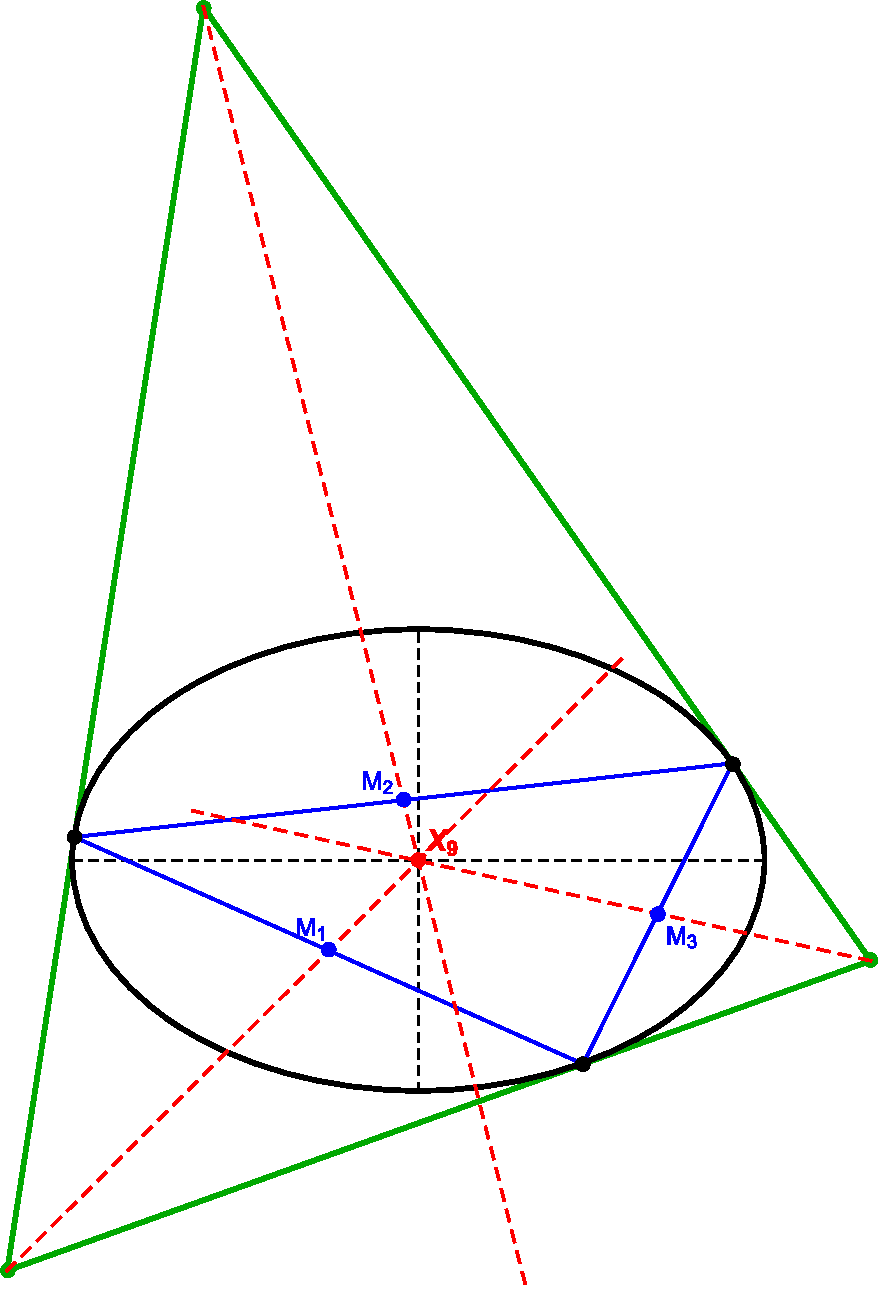
\includegraphics[height=1.75\linewidth]{pics/0051_mitten.pdf}
         \caption{An $N=3$ orbit (blue) and its Excentral Triangle (green), as well as the construction for $X_9$, the Mittenpunkt, located at the center of the Billiard (black).}
         \label{fig:mitten}
     \end{subfigure}
     \hfill
     \begin{subfigure}[t]{0.29\textwidth}
         \centering
         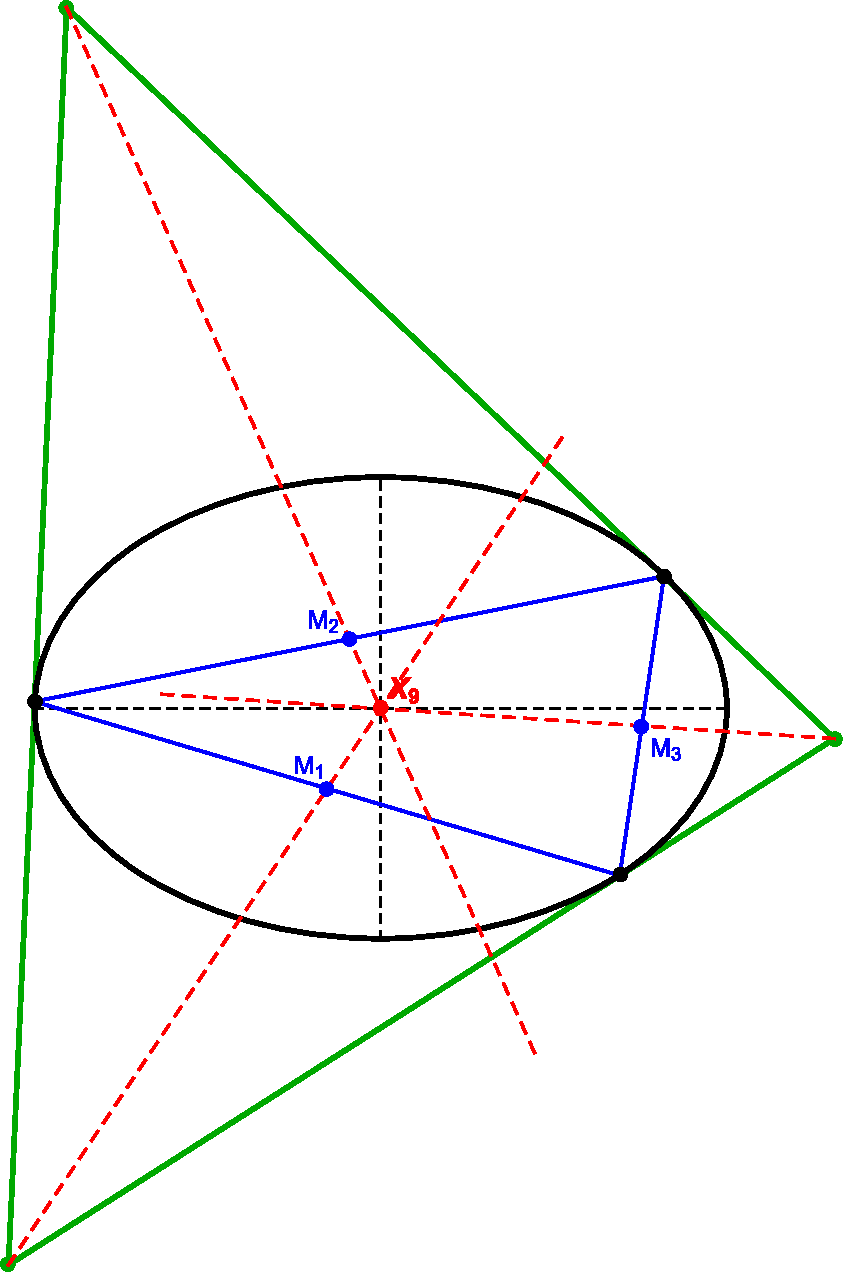
\includegraphics[height=1.75\linewidth]{pics/0052_mitten_rot.pdf}
         \caption{same construction for a slightly different orbit position, with $X_9$ unmoved.}
         \label{fig:mitten-rot}
     \end{subfigure}
     \hfill
     \begin{subfigure}[t]{0.29\textwidth}
         \centering
         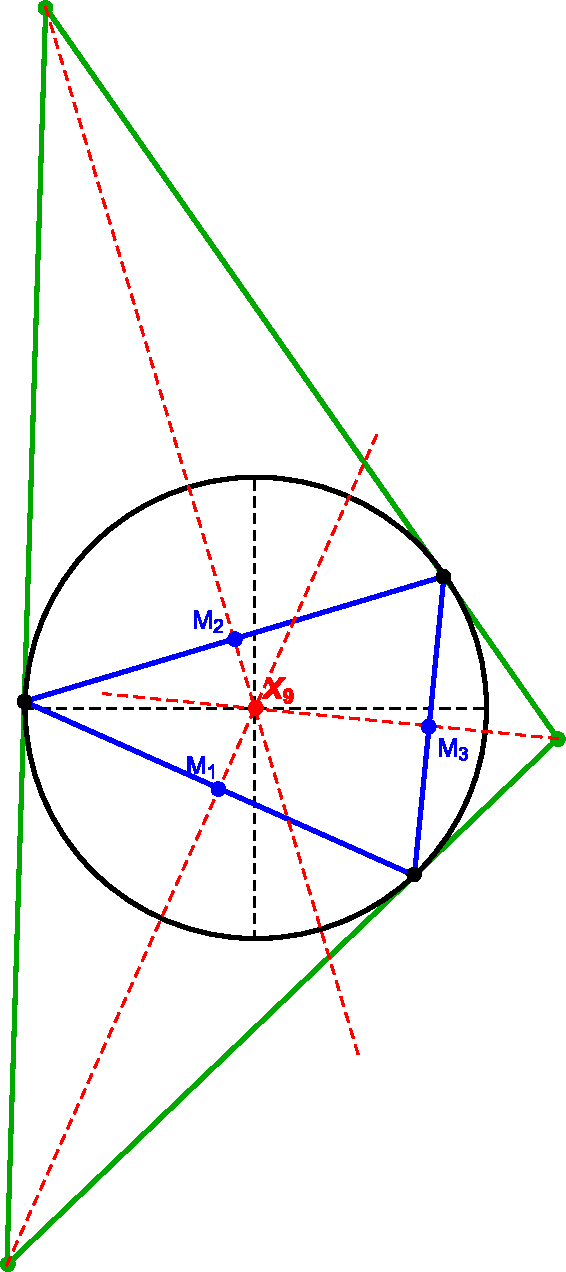
\includegraphics[height=1.75\linewidth]{pics/0053_mitten_rot_scaled.pdf}
         \caption{Affine transformation for which the Billiard becomes a circle, side midpoints become {\em chords} midpoints (distance ratios are preserved), and lines passing through transformed Excenters and chord midpoints concur at the circle center, uniquely identified under the transform with the Billiard center. 
         \label{fig:mitten-proof}}
     \end{subfigure}
     \caption{Left and Middle: Stationarity of the Mittenpunkt. Right: Proof via an Affine Transform.}
\end{figure}

\subsection{The Circumbilliard}

A triangle's {\em circumellipse} \cite{mw} passes through its three vertices. For $N=3$ orbits, we call this object a {\em Circumbilliard}. Since the orbit's Mittenpunkt $X_9$ is congruent with the Billiard's center, Figure~\ref{fig:circumbilliard}, we have:
%
\begin{observation}
Every triangle has a circumellipse to which it is a billiard orbit, whose center coincides with the triangle's Mittenpunkt.
\end{observation}
%
\begin{figure}[h]
    \centering
    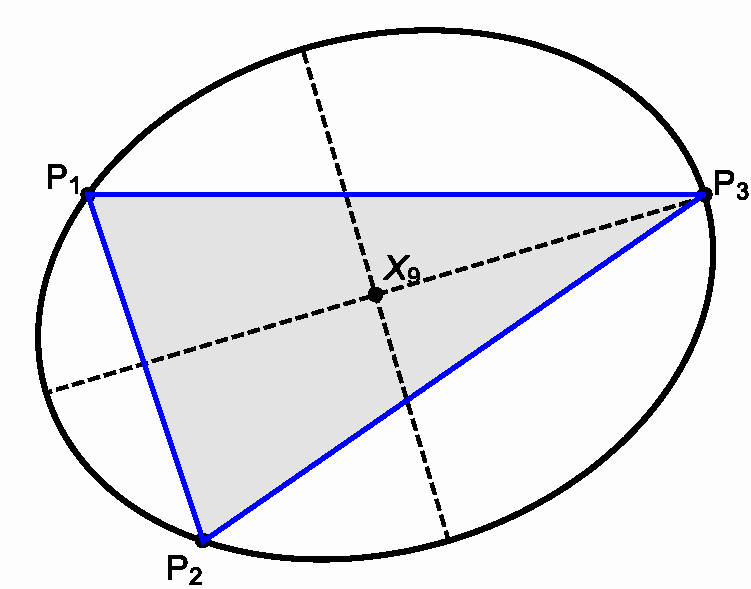
\includegraphics[width=.4\textwidth]{pics/0056_circumplot.pdf}
    \caption{A triangle's {\em Circumbilliard} is the circumellipse centered on $X_9$, the Mittenpunkt.}
    \label{fig:circumbilliard}
\end{figure}

\section{Can this Ratio be an Invariant?}
\label{sec:cosines}
An $N=3$ orbit, for being a triangle, will be associatd with a few ``famous'' circles: the Incircle, Circumcircle, and 9-Point Circle \cite{mw}. Denote their radii as $r$ (inradius) $R$ (circumradius) and $r_9$, respectively,  Figure~\ref{fig:radii}.

\begin{figure}[H]
    \centering
    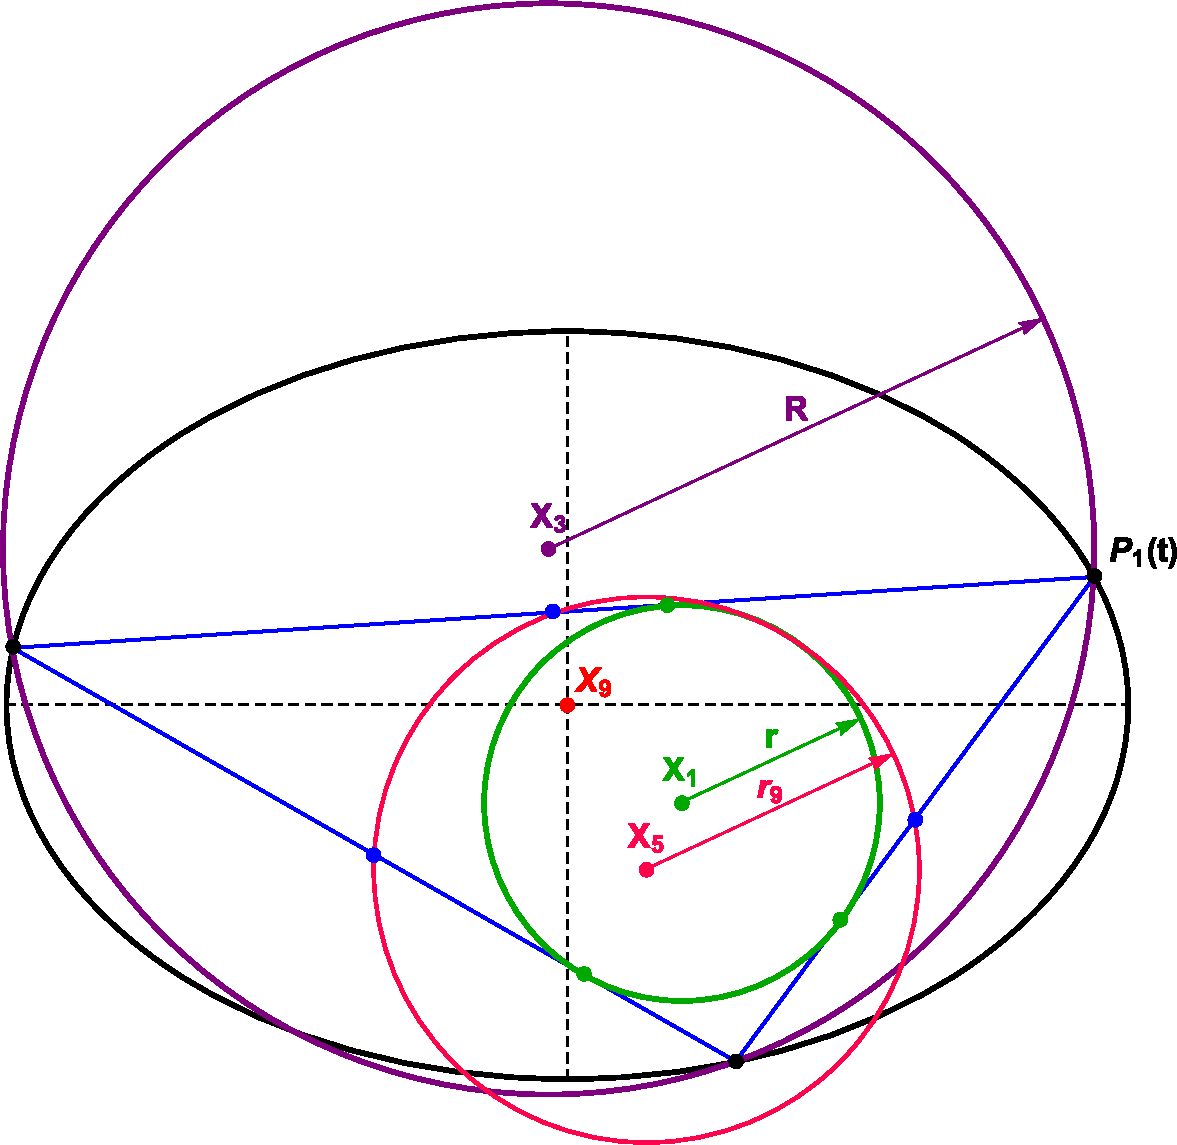
\includegraphics[width=.7\textwidth]{pics/0070_Radii.pdf}
    \caption{An orbit is shown (blue), whose leader vertex is $P_1(t)$. Shown also are its  Incircle (green), Circumcircle (purple), and 9-Point Circle (pink), with centers at $X_1$, $X_3$, and $X_5$. Their radii are the Inradius $r$, Circumradius $R$, and 9-Point Circle radius $r_9$.}
    \label{fig:radii}
\end{figure}

Inspecting the three notable radii against the parameter $t$ of $P_1$, Figure~\ref{fig:radii_plot}, one notices the known proportionality of $R=2r_9$ \cite{mw}. A remarkable fact is that $R$ is also proportional to $r$, as shown by a scatter plot Figure~\ref{fig:radii_scatter}, for any Billiard aspect ratio $a$. In fact \cite{ronaldo19a}:

\begin{equation}
\frac{r}{R}=\frac{2(\delta-1)}{(a^2-1)(\delta+a^2)}
\label{eqn:r-ov-R}
\end{equation}

Suprisingly, an alternate formula for $r/R$ has been derived \cite{dominique19,sergei19_private_circles} in terms of the perimeter $L$ and momentum $\gamma$:

\begin{equation}
    \frac{r}{R} = \gamma L - 4
    \label{eqn:rR_dominique}
\end{equation}

\begin{figure}[H]
    \centering
     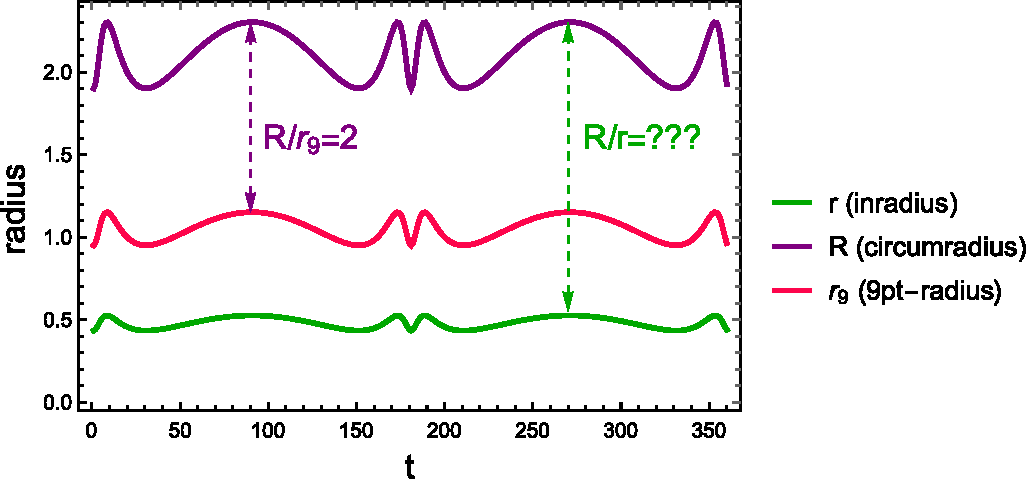
\includegraphics[width=.75\textwidth]{pics/0075_radii_plot.pdf}
    \caption{The three notable radii vs the angular parameter $t$ in $P_1(t)$. The ratio $R/r_9=2$ is known for any triangle. Suprisingly, $R/r$ is also constant over the $N=3$ orbit family.}
    \label{fig:radii_plot}
\end{figure}

\noindent Since both are constant, so must $r/R$ be, and:

\begin{theorem}
The ratio $r/R$ of Inradius to Circumradius is conserved for an $N=3$ orbit family and only depends on the Billiard's aspect ratio.
\label{obs:rovR}
\end{theorem}

As shown in Figure~\ref{fig:ratio_vs_a}, when $a=1$ (Billiard is circular), $r/R$ is maximal at $0.5$ (orbits are equilaterals). As $a\rightarrow\infty$, the ratio goes to zero. An inflection point occurs at $a\simeq{1.37}$, $r/R\simeq{.407}$, whose geometric meaning is not yet understood.

\begin{figure}[H]
    \centering
    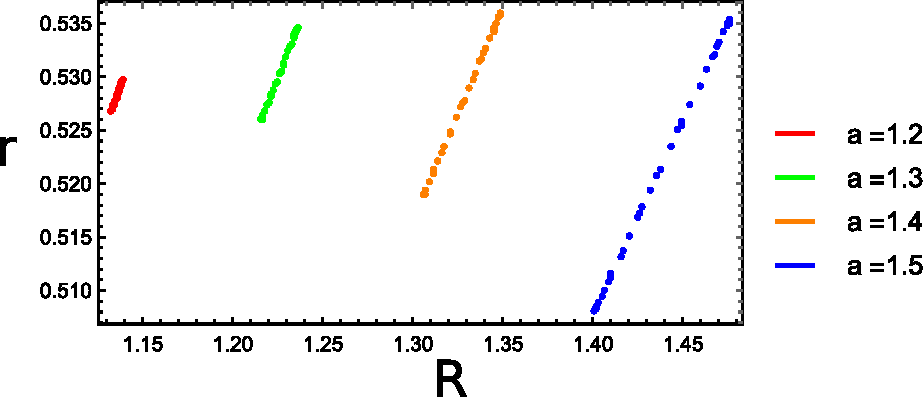
\includegraphics[width=0.75\textwidth]{pics/0080_radii_scatter.pdf}
    \caption{A scatter plot of Inradius vs Circumradius for various $t$ and various Billiard aspect ratios, showing linear dependence.}
    \label{fig:radii_scatter}
\end{figure}

\begin{figure}[H]
    \centering
    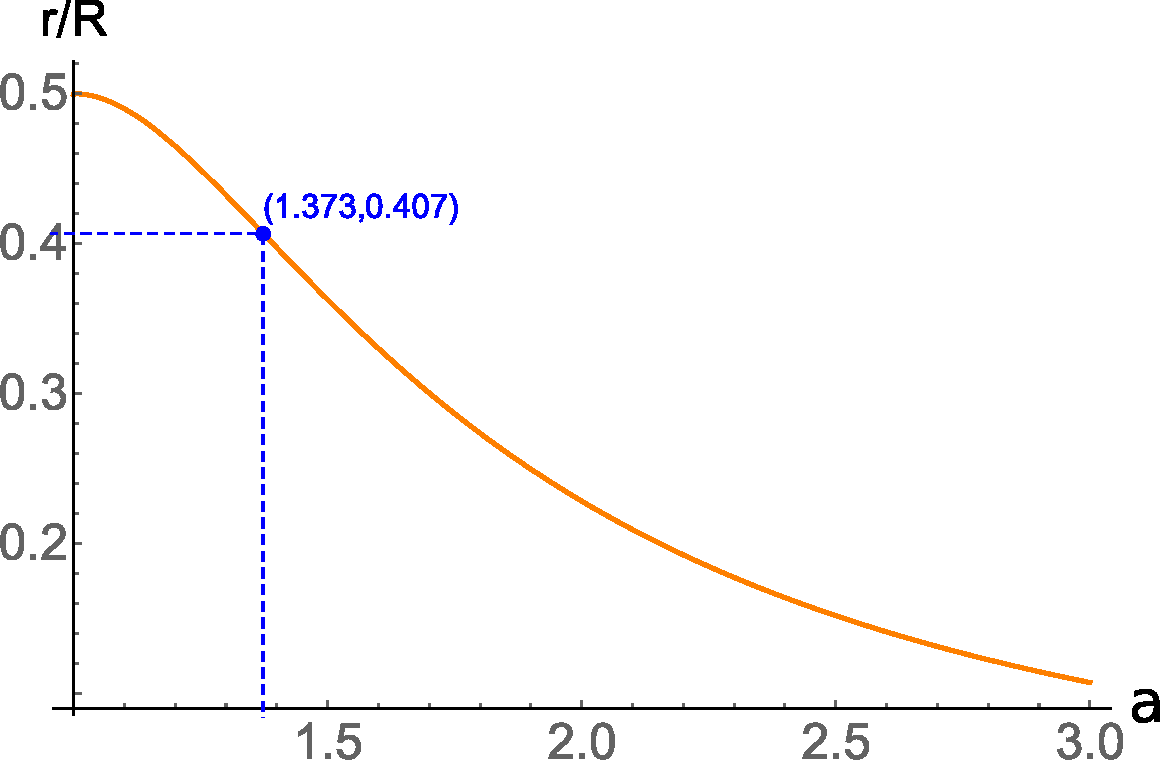
\includegraphics[width=.55\textwidth]{pics/0085_r_ov_R.pdf}
    \caption{The ratio $r/R$ as a function of the Billiard's axis ratio $a$ and an inflection point.}
    \label{fig:ratio_vs_a}
\end{figure}

\subsection{Conservation of the Sum of Cosines}

Denote $\theta_i,i=1,2,3$ the angles internal to the orbit. The following is a remarkable identity valid for any triangle \cite{johnson29}:

\begin{equation}
\sum_{i=1}^{3}{\cos\theta_i}=1+\frac{r}{R}
\label{eqn:rR_cos}
\end{equation}

Since the right-hand side is constant, so must be the sum of the cosines! These are shown against $P_1$'s parameter in Figure~\ref{fig:cosine_sum_n3}. Also shown is their their constant sum. So a corollary to Observation~\ref{obs:rovR} is:

\begin{corollary}
\label{cor8}
The sum of cosines is invariant for the $N=3$ family of orbits. 
\end{corollary}

\noindent Equations~\ref{eqn:rR_cos} and \ref{eqn:rR_dominique} imply
that the average cosine is given by:

\begin{equation}
\frac{1}{3}\sum_{i=1}^{3}{\cos\theta_i}=\frac{\gamma{L}}{3}-1
\label{eqn:rR_cos_avg}
\end{equation}

\begin{figure}[H]
    \centering
    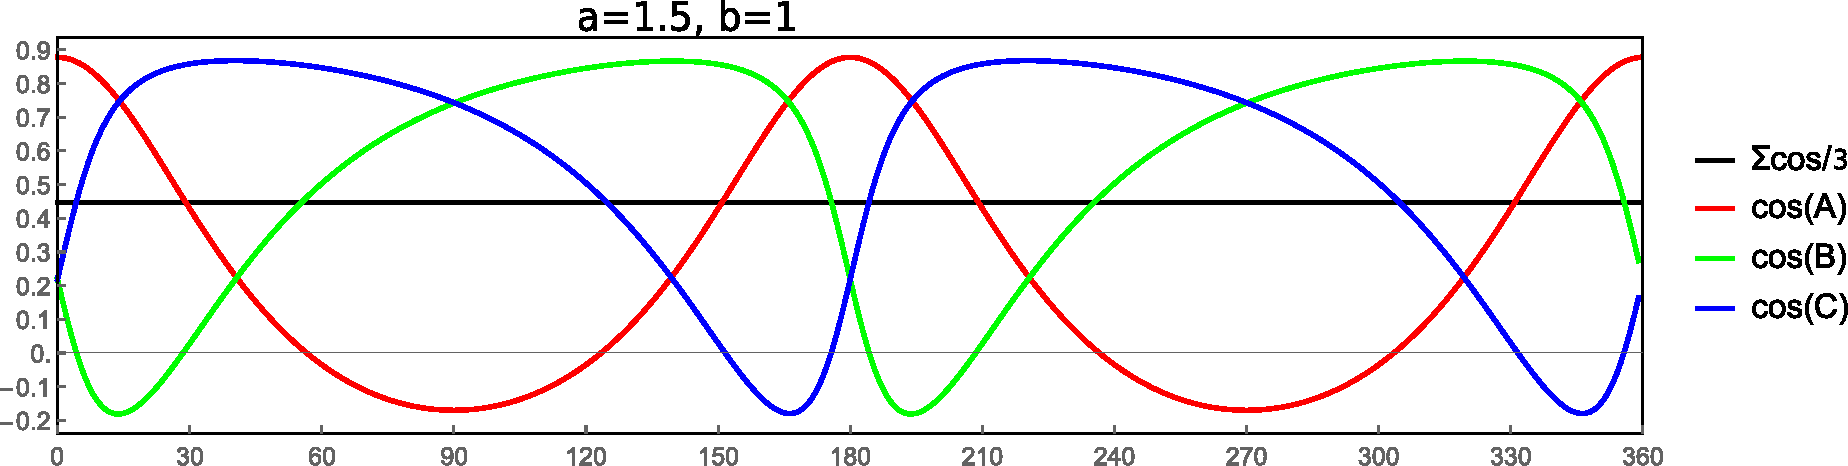
\includegraphics[width=\textwidth]{pics/0090_cosine_sum_n3.pdf}
    \caption{Cosines of each of orbit's internal angles (red, green, blue), as well as the arithmetic mean of their sum (black), showing constancy.}
    \label{fig:cosine_sum_n3}
\end{figure}

\subsection{Conservation of the Product of Excentral Cosines}

A triangle is always the Orthic of its Excentral \cite{mw}. If $\theta_i'$ are the Excentral's angles, the following is a known relation \cite{johnson29}:

\begin{equation}
\prod_{i=1}^{3}{|\cos\theta_i'|}=\frac{r}{4R}
\label{eqn:prod-cos}
\end{equation}

Let $\theta_i'$ be an angle of the Excentral Triangle opposite orbit angle $\theta_i$. It can be shown that $\theta_i'=\frac{\pi-\theta_i}{2}$, i.e., the Excentral Triangle is acute. Therefore the absolute sign in Equation~\ref{eqn:prod-cos} can be dropped. Since the right hand side of the above is constant:

\begin{corollary}
\label{cor9}
The product of cosines of Triangles Excentral to the $N=3$ orbit family is conserved.
\end{corollary}

\subsection{Conservation of Excentral-to-Orbit Area Ratio}

Let $A$ be the area of some triangle and $A_h$ the area of its Orthic. A known relation is \cite{johnson29}:

\begin{equation}
\frac{A}{A_h}=\frac{2R_h}{r_h}   
\end{equation}

Since the orbit is its Excentral's Orthic, $r/R$ constant implies:

\begin{corollary}
\label{cor10}
The Excentral-to-Orbit area ratio is constant and equal to $2R/r$.
\end{corollary}


\section{Can a Locus be a Circle?}
\label{sec:circles}
Loci can be elliptic, non-elliptic, or even a point. But can they be circular? And to boot, stationary?

Let $P$ be an orbit's vertex and $P'$ its reflection about the origin, also on $B$, 
Figure~\ref{fig:cosine_circle_construction}. Let  $Q_1$ and $Q_2$ be intersections of the tangent to $B$ at $P'$ with the orbit's Excentral Triangle $T'$. The following remarkable property is verified, illustrated in Figure~\ref{fig:cosine_circle_locus}: 


\begin{theorem}
The locus of $Q_1$ (or $Q_2$) is a {\em stationary circle}, and its center is the billiard's.
\end{theorem}

\begin{figure}[H]
     \centering
     \begin{subfigure}[t]{0.45\textwidth}
         \centering
         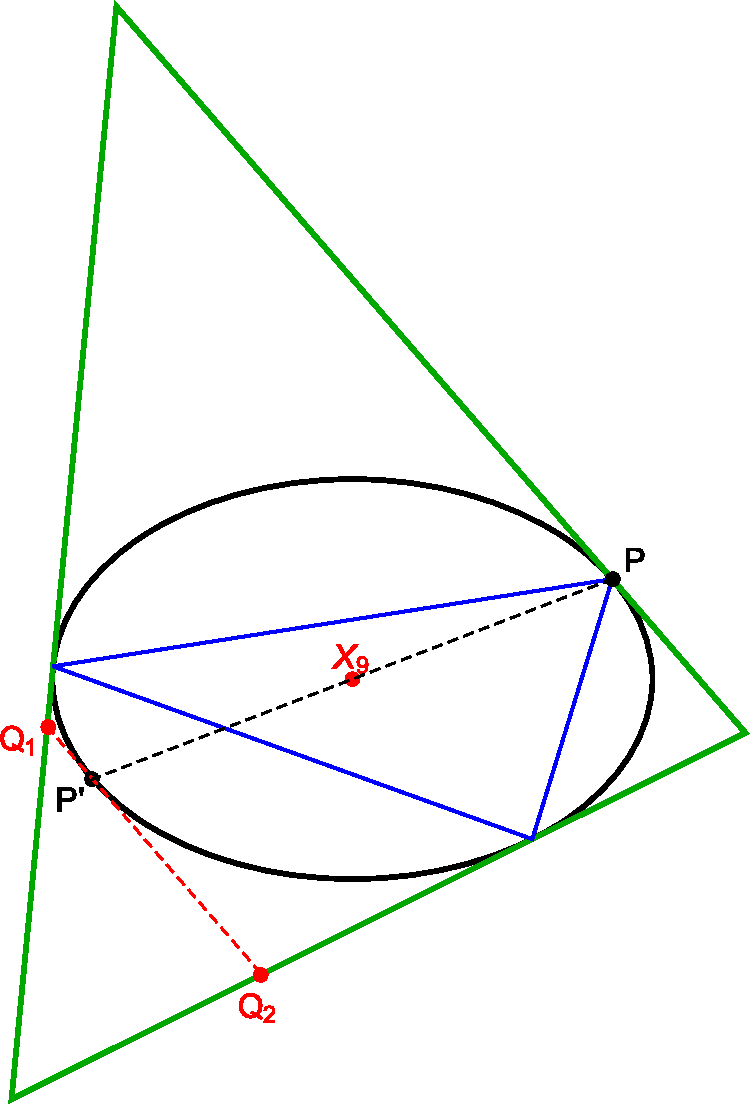
\includegraphics[width=1.0\linewidth]{pics/0100_cosine_circle_construction.pdf}
    \caption{Stationary Circle Construction.}
    \label{fig:cosine_circle_construction}
     \end{subfigure}
     \hfill
     \begin{subfigure}[t]{0.45\textwidth}
         \centering
          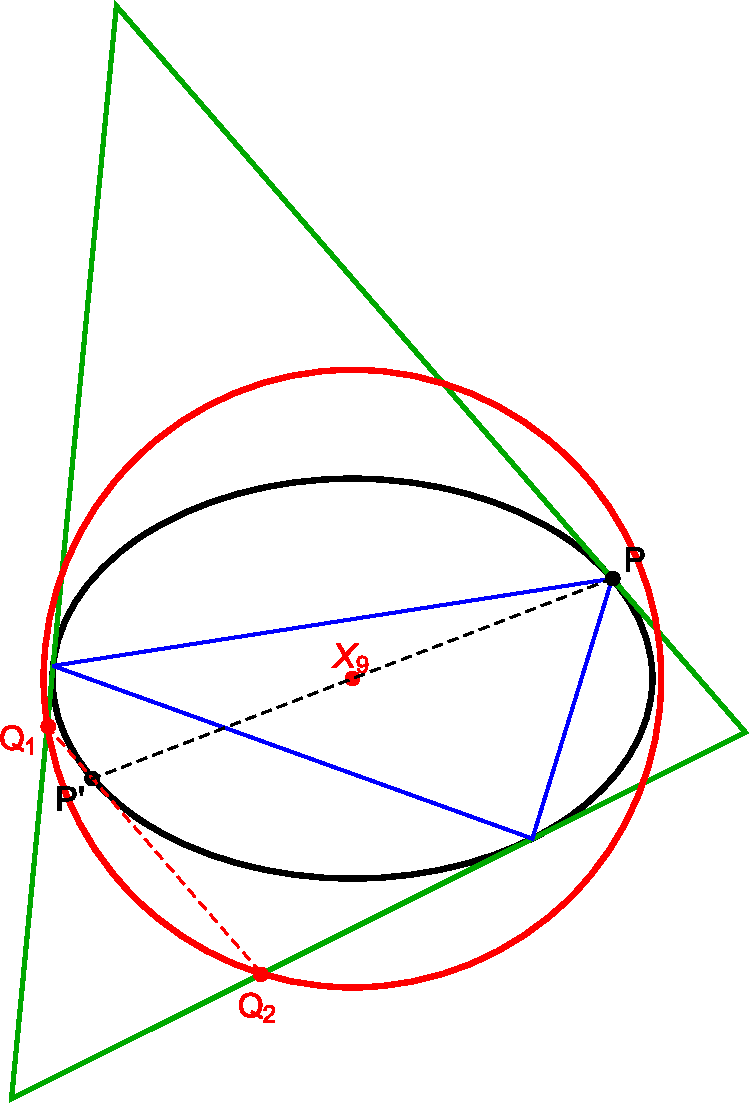
\includegraphics[width=1.0\linewidth]{pics/0110_cosine_circle_locus.pdf}
         \caption{Circular Locus of $Q_1$ (or $Q_2$).}
         \label{fig:cosine_circle_locus}
     \end{subfigure}
     \caption{Construction of Circular Locus.}
\end{figure}

The radius $r^*$ of this circle is given by \cite{ronaldo19a}:

\begin{equation}
r^* = \frac{\sqrt{3}}{3}\sqrt{2\delta+a^2+1}\,>\,a
\label{eqn:rstar}
\end{equation}

It turns out, the above locus is congruent with the {\em Cosine Circle} of the Excentral Triangle, also known as its {\em Second Lemoine Circle} \cite{mw}. Its center is known to lie on the Symmedian Pointof the Excentral, known to be congruent with the Mittenpunkt $X_9$, stationary in our case. The radius of the Cosine Circle can also be stated as a function of the constant perimeter $L$ and momentum $\gamma$ \cite{dominique19,sergei19_private_circles}:

\begin{equation}
    r^* = \frac{L}{\frac{r}{R}+4} = \frac{1}{\gamma}
\end{equation}

Also notable is the Excentral's {\em Cosine Hexagon} \cite{mw} whose six vertices are concyclic with the Cosine Circle \cite{mw}. Remarkably, its six sides will be either parallel to the orbit's or tangent to the billiard, Figure~\ref{fig:cosine_hexagon}. The vertices for the Excentral Cosine Hexagon can also be constructed by intersecting the orbit's Excentral Triangle with its copy reflected about the Billiard center, \ref{fig:cosine_circle_excentral_hexagon}

No other {\em Tucker Circles} \cite{mw} for the $N=3$ family have been found to be stationary.

\begin{figure}[H]
     \centering
     \begin{subfigure}[t]{0.45\textwidth}
         \centering
          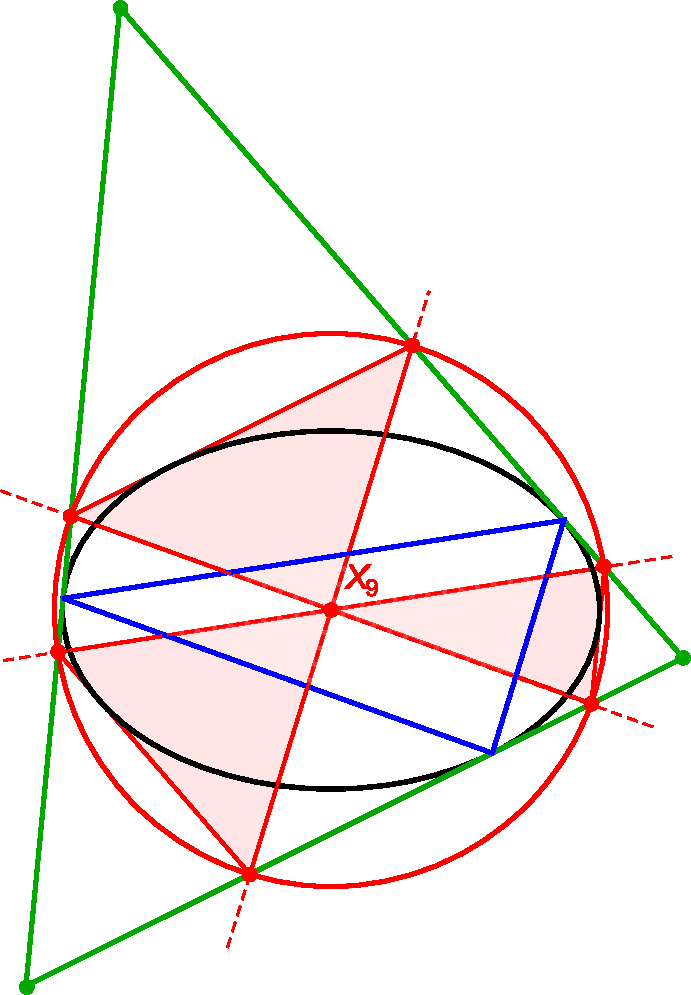
\includegraphics[width=1.0\linewidth]{pics/0130_cosine_hexagon.pdf}
         \caption{The vertices of the Excentral's Cosine Hexagon are the intersections of antiparallels (lines parallel to the Orthic, which in our case is the orbit) drawn through the Symmedian of the Excentral (congruent with the Mittenpunkt of the orbit and therefore stationary). These vertices are concyclic on the stationary Cosine Circle.}
     \label{fig:cosine_hexagon}
     \end{subfigure}
    \hfill
     \begin{subfigure}[t]{0.45\textwidth}
         \centering
         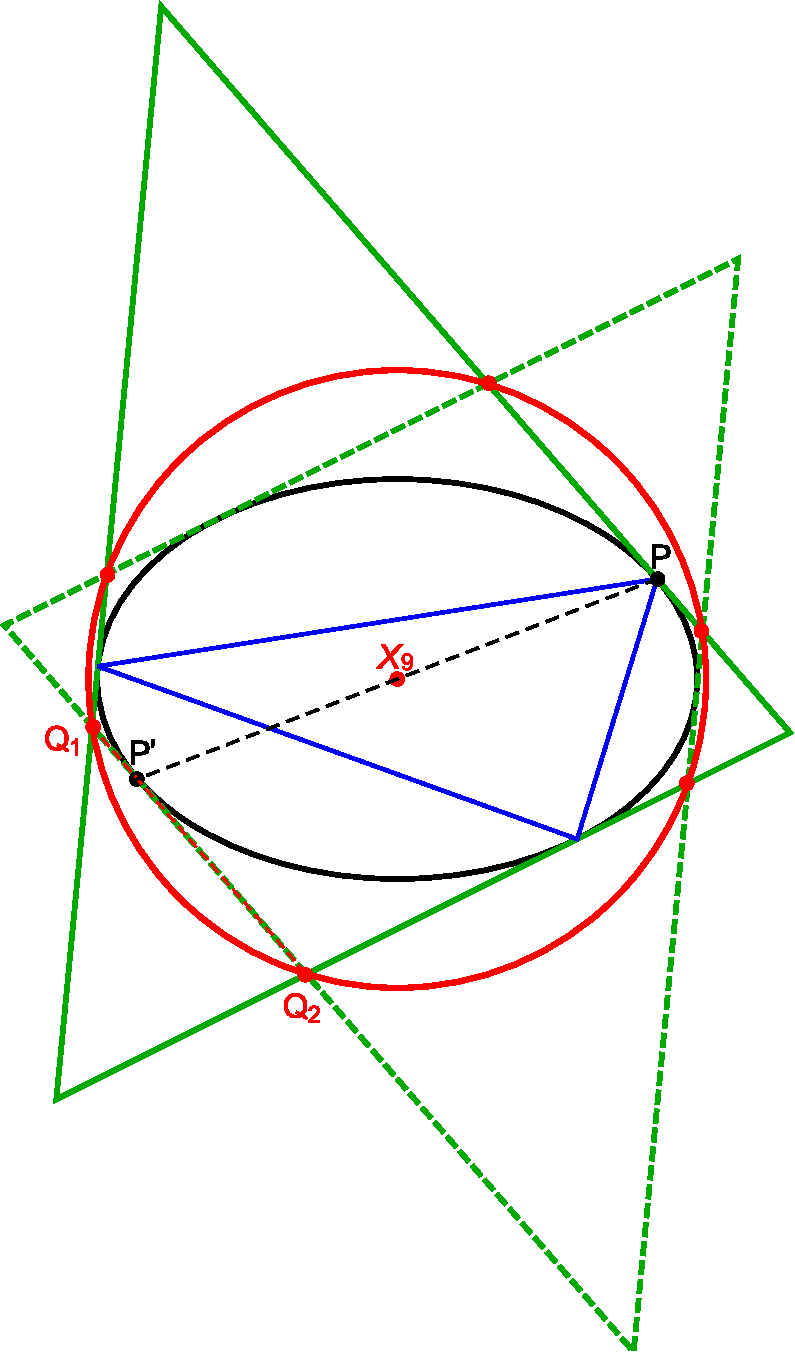
\includegraphics[width=1.0\linewidth]{pics/0120_cosine_circle_reflected_excentral.pdf}
    \caption{The Excentral Triangle intersects its reflection about the Symmedian on the six vertices of its Cosine Hexagon. Their locus is the Excentral's stationary Cosine Circle.}
    \label{fig:cosine_circle_excentral_hexagon}
     \end{subfigure}
     \caption{Two constructions for the concyclic vertices of the Excentral's Cosine Hexagon, whose locus is a stationary circle.}
\end{figure}

A video of this surprising phenomenon is available here \cite[video \#8]{dsr_main_videos_2019}.


\section{Monge Miracles: onward to $N>3$}
\label{sec:generalize}
If one searches for an ellipse's inscribed 4-gon of maximal perimeter, one finds the family of $N=4$ orbits which are all parallelograms \cite{connes07}. Their tangential polygons (tangent at the ellipse) are rectangles, and their vertices describe a circular locus, known as Monge's Orthoptic Circle \cite{mw}, Figure~\ref{fig:monge-orthoptic}:

Close observation of the above provided us with invaluable clues with which to generalize $N=3$ invariants to $N>3$ orbits. Namely:

\begin{itemize}
    \item Stationary Circle: The orthoptic locus is a stationary circle.
    \item Null Sum of Cosines: The polygon formed by the four tangency points is a parallelogram so the sum of its cosines is therefore zero.
    \item Null Product of Cosines: The Tangential Polygon is a rectangle and therefore the product of its cosines is zero.
    \item Mittenpunkt: The lines connecting the Tangential Polygon's vertices to the parallelogram midpoints concur at the Ellipse's center.
\end{itemize}

\subsection{$N>3$ Stationary Point}

For an $N=3$ orbit, the Mittenpunkt is where lines drawn from each Excenter through the sides' midpoints meet. As shown in Figure~\ref{fig:gen-mitten}, lines drawn from each vertex of the Tangential Polygon through the midpoint of the corresponding orbit side will meet at the stationary center of the Billiard. The same Affine Transform argument of Figure~\ref{fig:mitten-proof} can be used here, so we can state:

\begin{observation}
Consider an $N\geq{3}$ orbit family. The point of concurrence of lines from tangential vertices tangential through the orbit side midpoints is stationary at the center of the Billiard.
\end{observation}

\begin{figure}
    \centering
    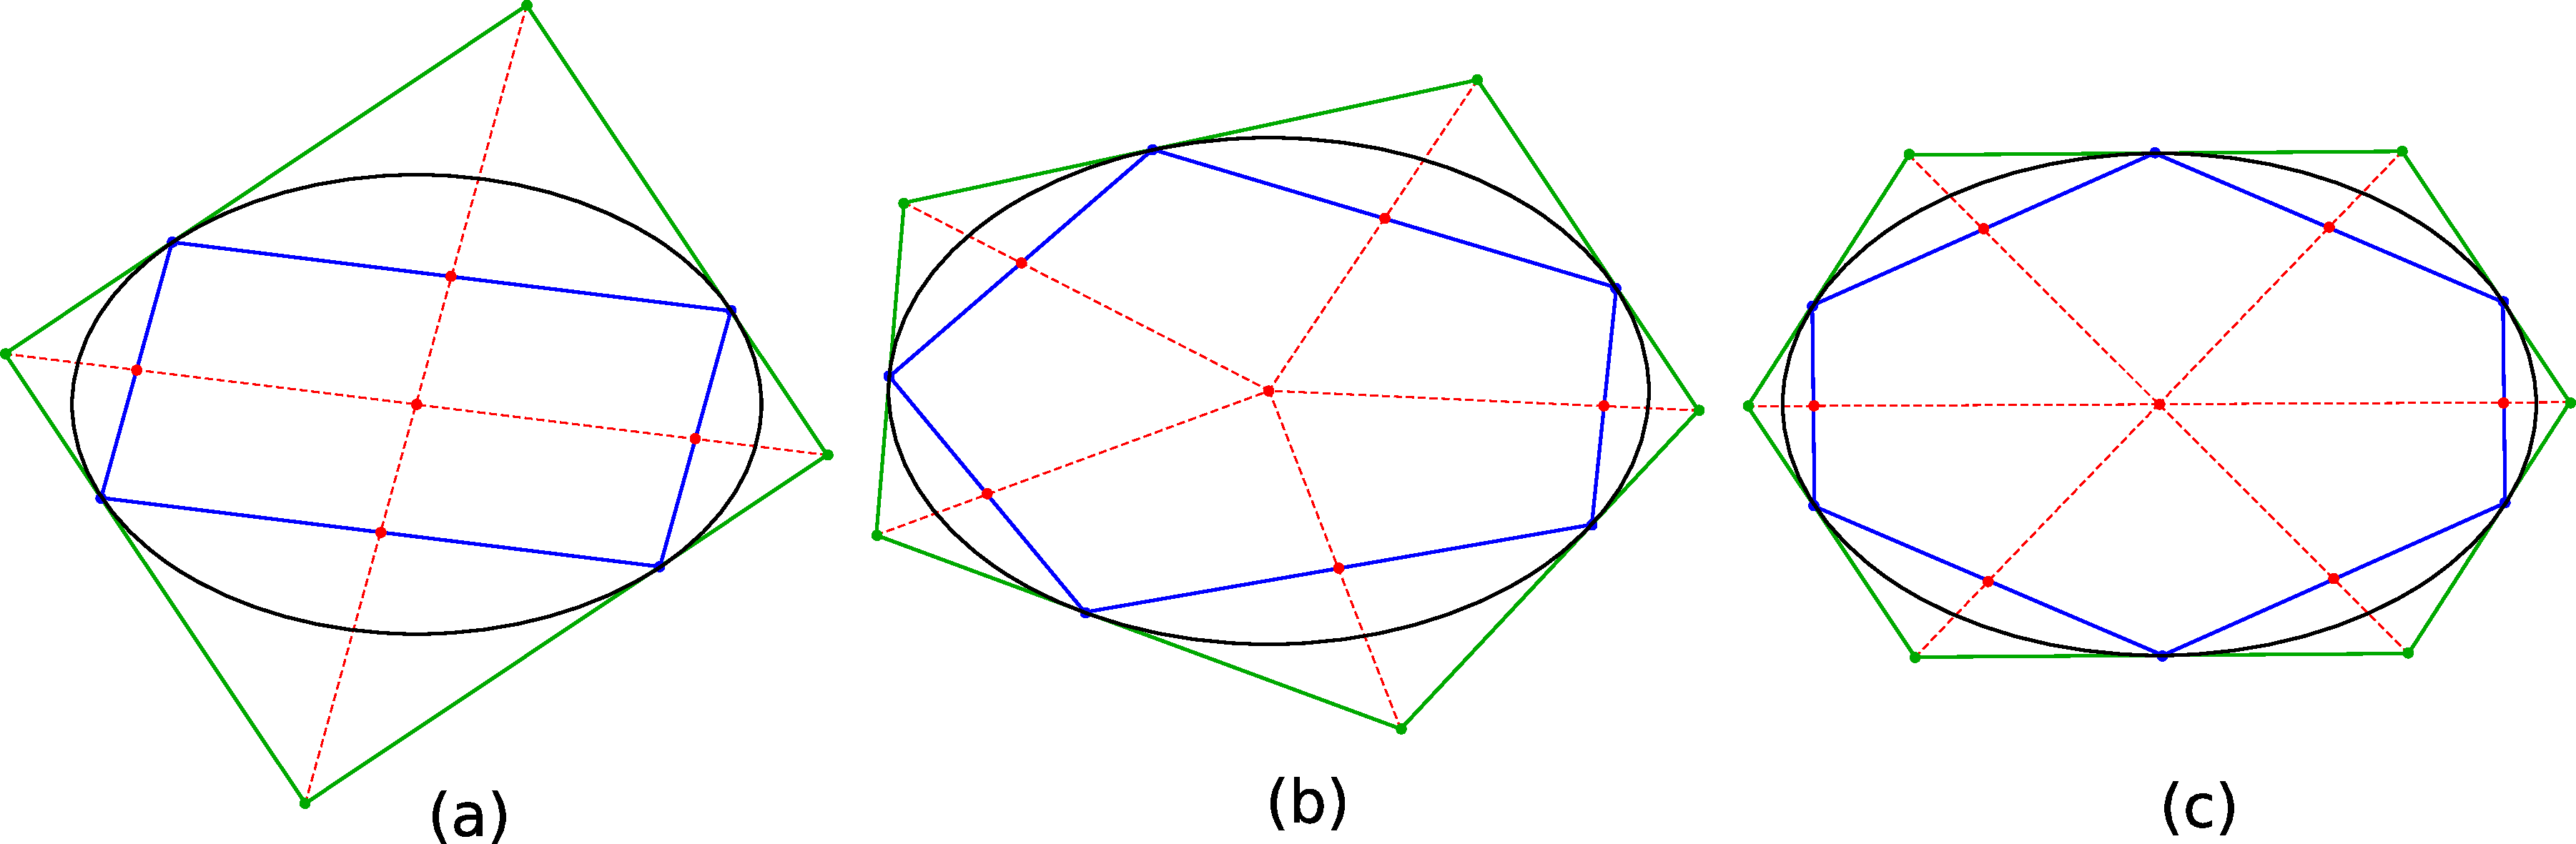
\includegraphics[width=\textwidth]{pics/0150_gener_mitten.pdf}
    \caption{Lines drawn from the vertices of an $N>3$ orbit's Tangential Polygon passing through the midpoint of the corresponding orbit sides meet at the stationary center of the Billiard.}
    \label{fig:gen-mitten}
\end{figure}

\subsection{$N>3$ Cosine Sum and Product}

The fact that both $N=3$ and $N=4$ conserve cosine sum, suggests $N>4$ might as well, and this was first confirmed numerically for $N=5,..30$ non-intersecting orbits at various Billiard aspect ratios. Figure~\ref{fig:gen-cos-sum-n45} shows cosine curves adding to a constant for $N=4,5$ with $a=1.5$.

The following elegant proof has been kindly contributed \cite{sergei19_private_meromorphic}. Using Equation~\ref{eqn:joachim} the half-angle cosine in terms of momentum and length of gradient, and then with $\cos{t}=2\cos(t/2)^2-1$ write an expression for the sum of full-angle cosines:

\begin{eqnarray}
\cos\frac{\theta_i}{2} & = & \frac{\gamma}{|\nabla{f_i}|}\\
\sum_{i=1}^{N}{\cos\theta_i} & = & 2\,{\gamma}\sum_{i=1}^{N}\frac{1}{|\nabla{f_i}|^2}-N
\label{eqn:cosine-sum}
\end{eqnarray}

\noindent where $f_i=f(P_i)$. Then complexify the space and show that the poles of Equation~\ref{eqn:cosine-sum} on the elliptic curve covering the conic cancel each other. So one has a pole-free meromorphic function, hence a constant.

\begin{theorem}
The sum of cosines is conserved for non-intersecting orbits, $\forall{N}$.
\end{theorem}

\begin{figure}[H]
    \centering
    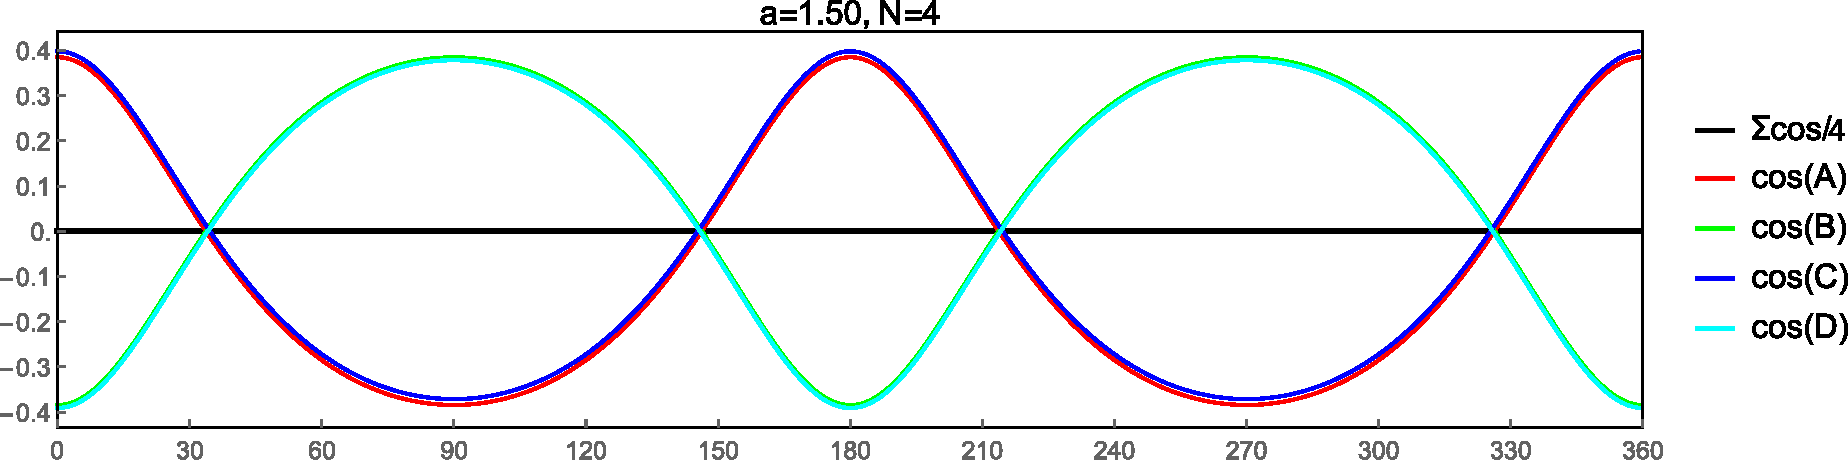
\includegraphics[width=\textwidth]{pics/0091_cosine_sum_n4.pdf}
    %
    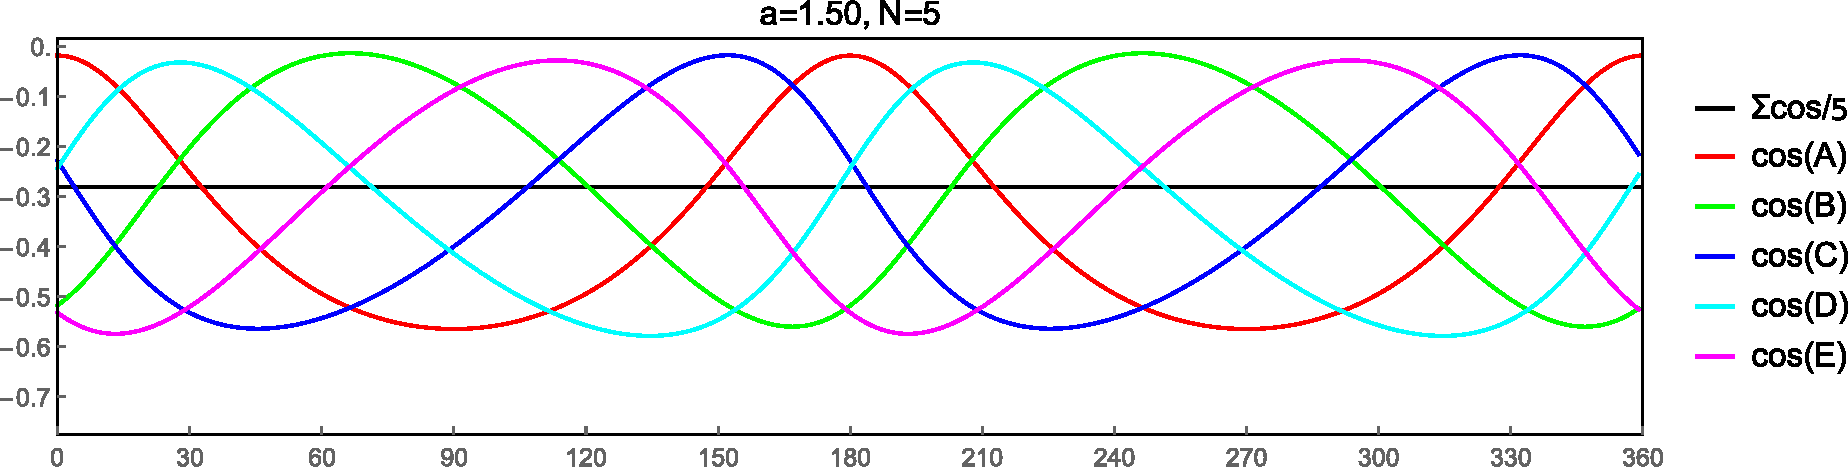
\includegraphics[width=\textwidth]{pics/0092_cosine_sum_n5.pdf}
    \caption{Individual cosine values are shown for the $N=4$ (top) and $N=5$ (bottom) family of orbits, $a=1.5$, vs. the parameter of a leader vertex. $N=4$ orbits are parallelograms, so opposite angles are supplementary and cosine curves are superimposed and symmetric, adding to zero. In the more asymmtric $N=5$ case, the 5 cosines still add to a constant value (black line at the bottom of the graph).}
    \label{fig:gen-cos-sum-n45}
\end{figure}

\begin{figure}[H]
    \centering
    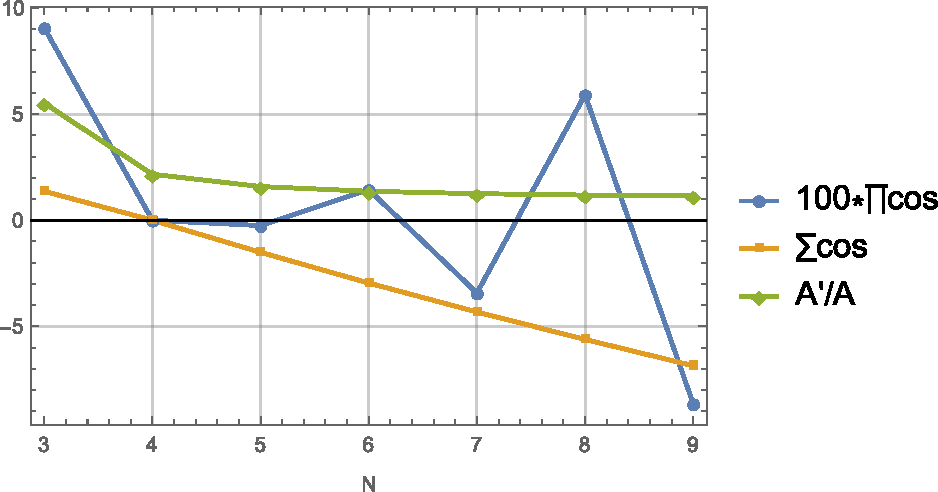
\includegraphics[width=\textwidth]{pics/0160_gener_prod_sum_area.pdf}
    \caption{Constant orbit cosine sum, tangential polygon cosine product (the latter is multiplied by a 100 to be visible), and tangential-to-orbit area ratio vs. $N$ for $a=1.5$.}
    \label{fig:gen-prod-sum}
\end{figure}

Similarly, since both $N=3$ and $N=4$ conserve the product of their Excentral/Tangential cosines, we verify numerically that $N=5,..30$ non-intersecting orbits at various aspect ratios also conserve this quantity. A proof to which (with similar techniques) has been kindly shared with us \cite{sergei19_private_meromorphic}.

\begin{theorem}
The product of cosines for non-intersecting orbits for {\em any} $N$ is conserved.
\end{theorem}

When trajectories are not closed, the sum of their cosines (resp. product of their excentral cosines) may be unbounded. One can then talk about the arithmetic mean (resp. geometric mean) of cosines for open trajectories (resp. their external tangents). In the Appendix we show how special spatial integrals can compute them, showing perfect match with the case when trajectories are closed orbits.

\subsection{Area Ratio for $N>3$}

For $N=3$ the Excentral-to-Orbit area ratio is conserved, however, we can easily check numerically that $N=4$ does not preserve the ratio of its rectangular Tangential-to-Orbit polygons.

Proceeding to $N>4$ we verify that only odd $N$ preserve area ratio, a fact which has been subsequently formally proven \cite{sergei19_private_meromorphic}. 
Figure~\ref{fig:gen-prod-sum} shows cosine sum, cosine product, and area ratio invariants for $N=3,4,\ldots,9$.

\begin{theorem}
The ratio of areas between Tangential Polygon and Non-Self-Intersecting Orbit is conserved for all odd $N$.
\end{theorem}

\subsection{Stationary $N>4$ Circles}

For the $N=3$ case,  Figure~\ref{fig:cosine_hexagon}(b), the locus of the intersection of an edge in the Excentral Triangle with an alternate edge reflected about the Billiard center is a stationary circle. For $N=4$ we have Monge's Orthoptic Circle. Can these two constructions be harmonized and extended to $N>4$? Indeed it can, in this surprising way:

\begin{theorem}
Let $O$ be the center of the Billiard. The locus of the intersection of an edge of the Tangential Polygon with the reflection of the next tangential edge about $O$ is a stationary circle centered on $O$. Its radius is $r^*=1/\gamma$, i.e., the inverse of angular momentum.
\end{theorem}

\noindent {\bf Proof} \cite{sergei19_private_circles}: Let $f$ be as in Equation~\ref{eqn:f}. $f_X$ represent $f(X)$. Consider two consecutive vertices $P$ and $Q$ of the orbit. Then:

\begin{itemize}
\item By momentum conservation $\hat{v}.\nabla f_P= -\hat{v}.\nabla f_Q=\gamma$. So we have:

\begin{equation}
    \hat{v}.\left(\nabla{f_P} + \nabla{f_Q}\right)=0
    \label{eqn:sum-nablas}
\end{equation}

\item Since $\nabla{f_P}$ (resp. $\nabla{f_Q}$) is normal to the ellipse at $P$ (resp.  $Q$), a point $z$ on the tangent line at $P$ (resp. $-Q$) is given by $z.\nabla{f_P}=1$ (resp. $z.\nabla{f_Q}=-1$).
\item Let $z$ be where both lines intersect, $z.\left(\nabla{f_P}+{\nabla} f_Q\right)=0$.

\item It follows from Equation~\ref{eqn:sum-nablas} that $z$ is proportional to $\hat{v}$.

\item Since $\hat{v}.\nabla{f_P}=\gamma$ and $z.\nabla{f_P}=1$, we have $z = \hat{v}/\gamma$.
\item That is, $z$ lies on the circle of radius $1/\gamma$.\qed
\end{itemize}

\noindent The radius of the stationary circle is plotted against the aspect ratio of the Billiard for a range of $N$ in Figure~\ref{fig:stationary-radius-vs-a}. The stationary circle is shown around various $N$ in  Figure~\ref{fig:gen-circ-grid} .

\begin{figure}
    \centering
    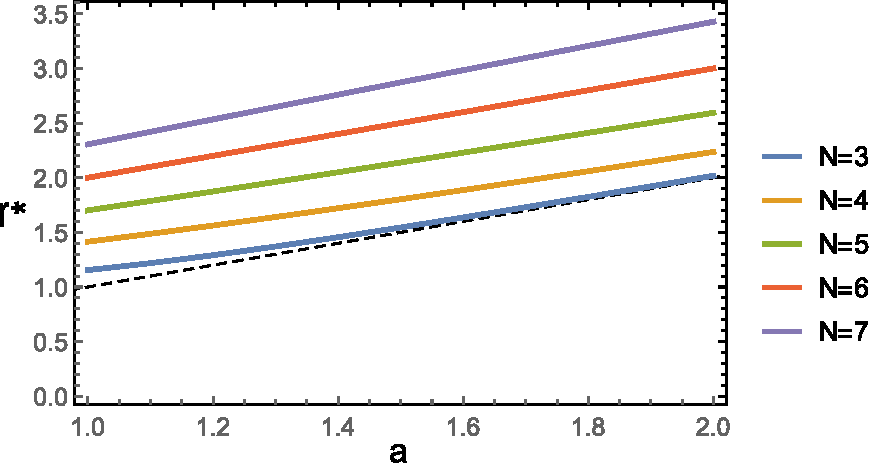
\includegraphics[width=.75\textwidth]{pics/0190_rstar.pdf}
    \caption{Radius of stationary circle vs $a$, for different values of $N$. A $x=y$ dashed line is drawn to show that for $N=3$, $r^*>a$.}
    \label{fig:stationary-radius-vs-a}
\end{figure}

\begin{figure}[H]
    \centering
    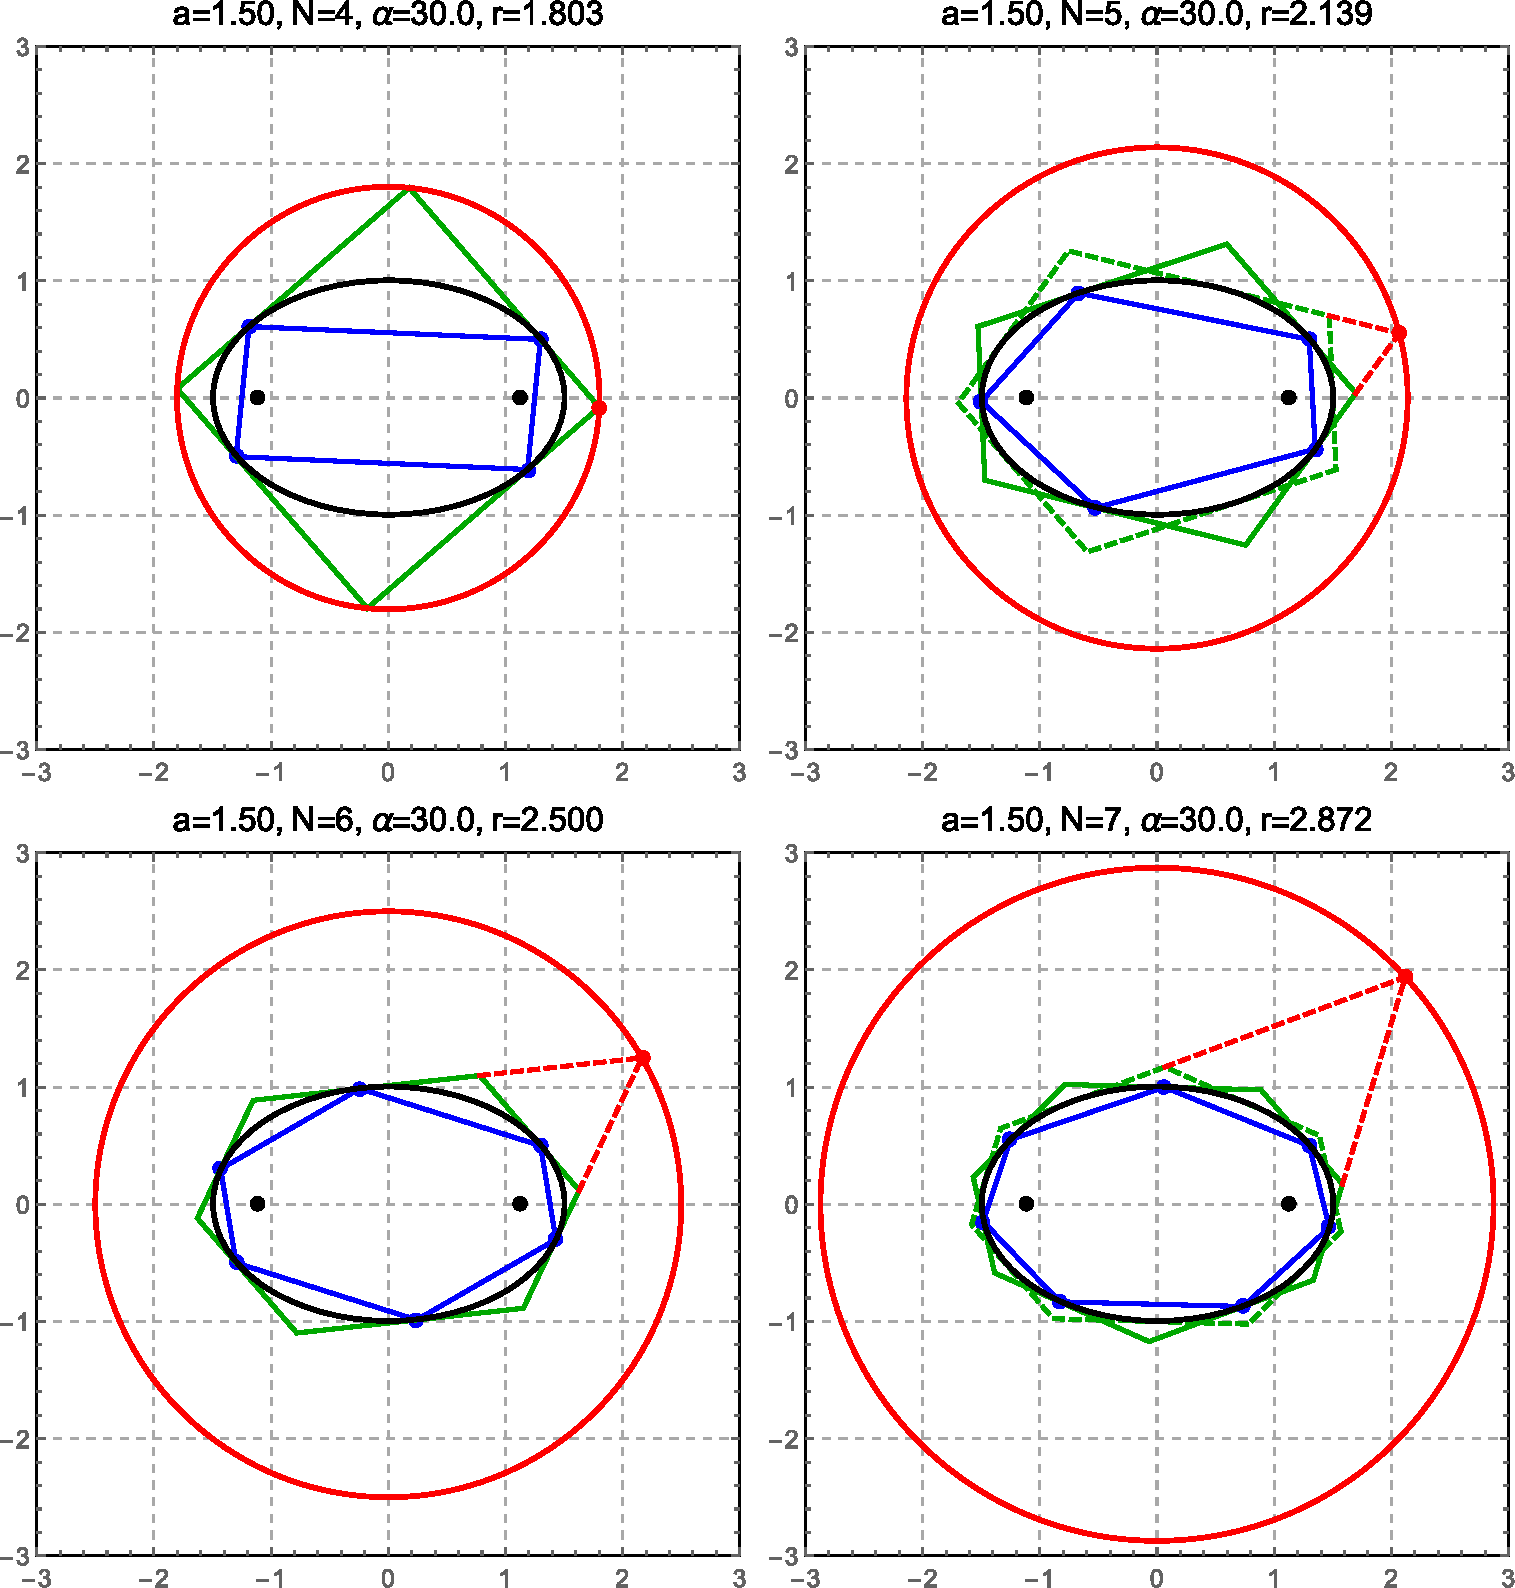
\includegraphics[width=\textwidth]{pics/0180_circ_grid.pdf}
    \caption{The loci of the intersection of an edge of the Tangential polygon with its reflection about the Billiard's center is a stationary circle for all $N$.}
    \label{fig:gen-circ-grid}
\end{figure}

\subsection{Summary}

The generalizations to $N>3$ found in this section are summarized on Table~\ref{tab:generalize}.

\begin{table}[H]
\caption{Generalizations of $N=3$ Invariants to $N>3$. Below $\theta_i,A,E_i$ refer to internal angle, area, or edge of the orbit polygon. When primed, they refer to the Tangential Polygon quantities. As before, $\delta=\sqrt{a^4+a^2-1}$.}
\label{tab:generalize}
$$
\begin{array}{r|c|c}
N=3~\mbox{Invariant} & N=3\,\mbox{Formula} & N\geq3\,\mbox{Invariant}  \\
\hline
\mbox{Perimeter L}&\frac{2(\delta+a^2+1)\sqrt{2\delta-a^2-1}}{a^2-1}&\mbox{Perimeter L}\\
\mbox{Angular Momentum}\,\gamma&\frac{\sqrt{2\delta-a^2-1}}{a^2-1}&\mbox{Angular Momentum}\\
\mbox{Mittenpunkt}\,X_9 & O & \mbox{Tang. medians meet at}\,O \\[5pt]
\frac{r}{R}=-1+\sum_{i=1}^3{\cos\theta_i} & \frac{2(\delta-1)}{(a^2-1)(\delta+a^2)} & \sum_{i=1}^N{\cos\theta_i} \\[5pt]
\prod_{i=1}^{3}{\cos\theta_i'} & \frac{r}{4R} & \prod_{i=1}^N{\cos\theta_i'} \\[5pt]
A'/A & \frac{2R}{r} & \forall{N}\mbox{ odd},A'/A\\[5pt]
\mbox{Radius of Cosine Circle }r^* &
    \frac{\sqrt{3}}{3}\sqrt{2\delta+a^2+1} & \mbox{Radius of }\,E'_i\cap-E'_{i+1},\,r^*=\frac{1}{\gamma}
\end{array}
$$
\end{table}

\section{Conclusion}
\label{sec:conclusion}
The old Elliptic Billiard did reveal to us a few more of its secrets. In a way it is like a cat: it never does what it is asked to do. But whatever it does is beautiful and surprising. Starting with the loci of triangular centers, you get a menu of elliptic, non-elliptic, and quasi-elliptic curves. Some are similar, others indentical to Billiard or Caustic. One is perfectly circular, another point-like.

Any combination of well-known invariants will produce another invariant. One surprise is that for $N=3$ the product of perimeter and angular momentum is manifested visibly as the constant ratio of Inradius to Circumradius. Equivalently, as constant orbit cosine sum, tangential cosine product, and tangential-to-orbit area ratios. Remarkably, all $N=3$ properties are also verified $\forall{N}$ (area ratios are only true for odd $N$). We leave the reader with a few questions:

\begin{itemize}
    \item For $N=3$, what determines whether a triangular center or vertex will produce an elliptic vs some other type of locus?
    \item Are there ellipsoidal (3d) counterparts to these invariants?
    \item Which invariants are still true for self-intersecting orbits?
    \item Are there non-Euclidean invariants?
\end{itemize}

\begin{acknowledgements}
We would like to thank Professors Sergei Tabachnikov, Richard Schwartz, Arseniy Akopyan, Olga Romaskevich, and Igor Minevich for invaluable mentoring, and key proofs. We would like to thank Paulo Ney de Souza and Prof. Jorge Zubelli for arranging our IMPA talk on July 31, 2019 \cite{impa2019} and Prof. Marcus Craizer for inviting us for a talk at PUC-RJ. We would like thank Mark Helman for contributing proofs for the ellipticity of several triangular centers \cite{helman19}.
\end{acknowledgements}

\appendix
\section{Appendix: Further Locus Phenomena}
\label{sec:locus-phenomena}
\subsection{Suprising Symmedian}

Interestingly, the Symmedian Point $X_6$ is the only triangular center out of Kimberling's first 12 whose locus is non-elliptic, though just by a smidgen: for an $a=1.5$ Billiard, the average error with respect to the best fit ellipse is of the order of $10^{-4}$, i.e., imperceptible to the naked eye. Figure~\ref{fig:symmedian} shows the locus of $X_6$ with the deviation from a perfect ellipse exaggerated a million-fold. In fact \cite{ronaldo19a}:

\begin{observation}
The locus of the Symmedian Point $X_6$ of an $N=3$ orbit is a convex quartic.
\end{observation}

\begin{figure}[H]
    \centering
    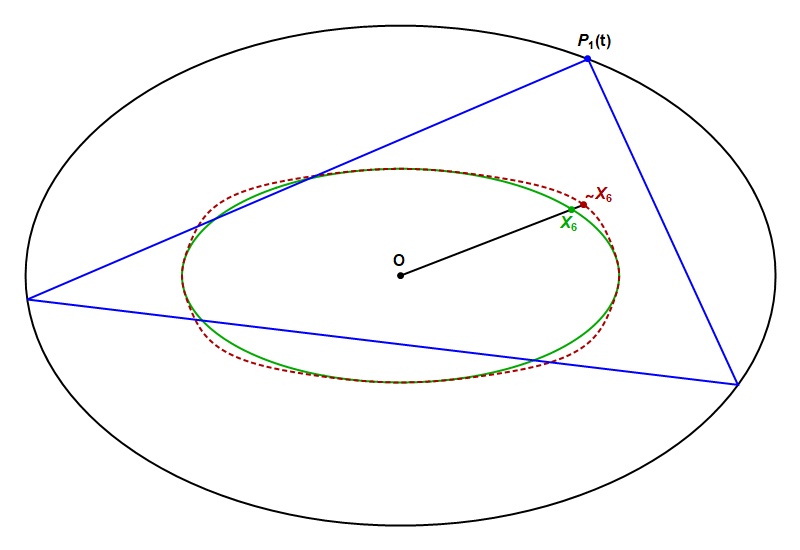
\includegraphics[width=.75\textwidth]{pics/0041_symmedian.png}
    \caption{The convex, quartic locus of the Symmedian Point $X_6$ (green), indistinguishable to the naked eye from an ellipse. The dashed red path shows the locus with the error with respect to a best-fit ellipse exaggerated a million-fold.}
    \label{fig:symmedian}
\end{figure}

\subsection{One Kinky Locus}

The locus of the Orthocenter $X_4$ is elliptic and similar to a rotated copy of the Billiard \cite{ronaldo19a}. At a particular aspect ratio $a_1\simeq{1.51}$, the locus is identical to the Billiard.

Another notable threshold is $a_0\simeq{1.352}$. A choice of $a<a_0$ (resp. $a>a_0$) will result in an orbit family without (resp. with) obtuse triangles, Figure~\ref{fig:orthocenter_loci}. 

\begin{figure}[H]
    \centering
    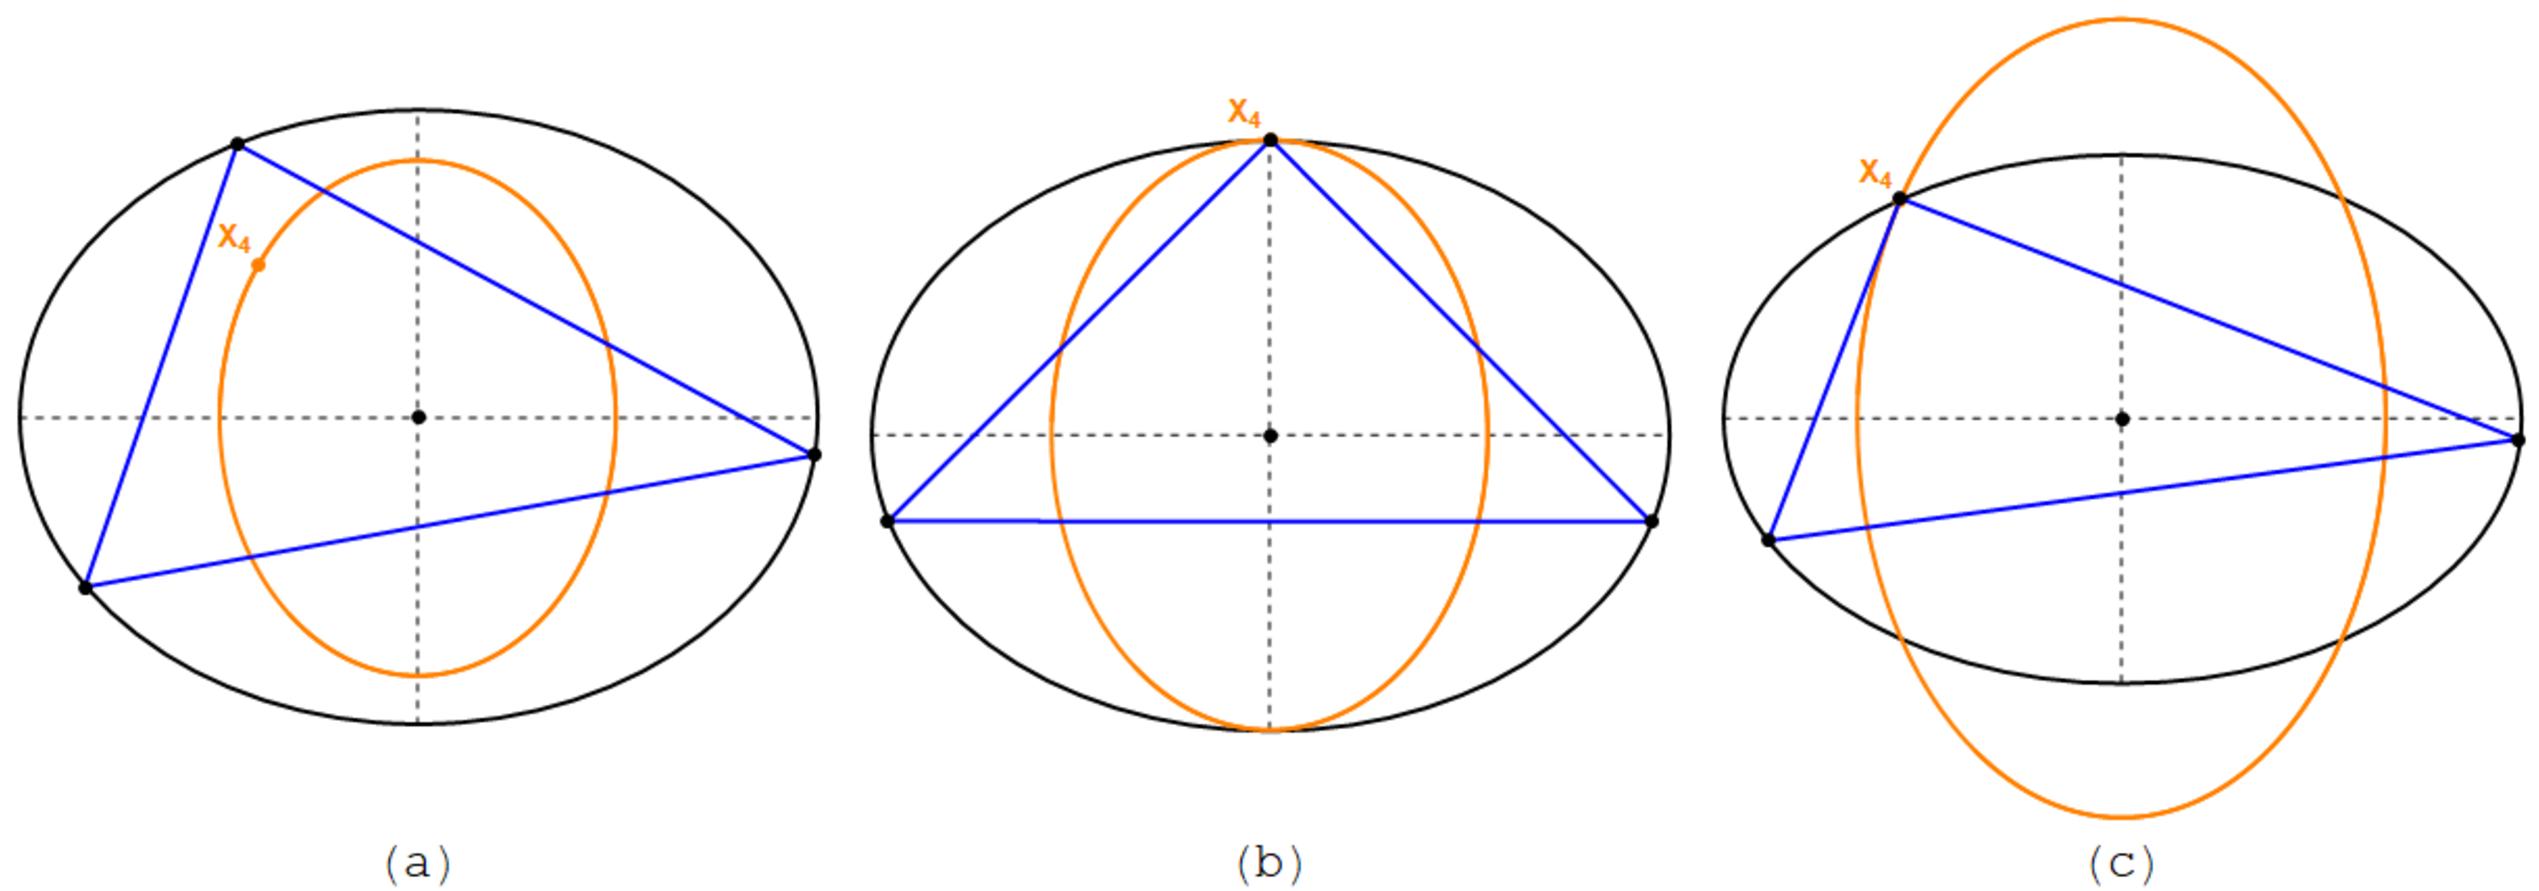
\includegraphics[width=\textwidth]{pics/0045_ort_loci.pdf}
    \caption{Let $B$ be the Billiard (black), $H$ the locus of the orthocenter $X_4$ (orange), and $a_0\simeq{1.352}$. (a) $a<a_0$: $H$  is within $B$ and orbits (blue) can never be obtuse. (b) $a\simeq{a_0}$: $H$ is tangent to $B$ at its top and bottom vertices. An orbit is a right triangle when any of its vertices is at said locations. (c) $a>a_0$: $H$ intersects $B$ on four points. When $X_4$ is inside (resp. outside) $B$, the orbit is acute (resp. obtuse).}
    \label{fig:orthocenter_loci}
\end{figure}

Assume now $a>a_0$ and that $T_h$ is the orbit's {\em Orthic Triangle} \cite{mw}. The Incenter $I_h$ of $T_h$ will display a {\em switching} behavior \cite{coxeter67}:

\begin{center}
\begin{tabular}{r|l}
 orbit & $I_h$ location \\ 
 \hline
 acute & orthocenter $X_4$ \\  
 obtuse & obtuse vertex 
\end{tabular}
\end{center}

At the current choice of aspect ratio, the orbit will be at times acute and obtuse, and the result is the locus of $I_h$ becomes piecewise elliptic, Figure~\ref{fig:orthic_incenter_locus} and \cite[video \#6]{dsr_main_videos_2019}.

\begin{figure}[H]
    \centering
    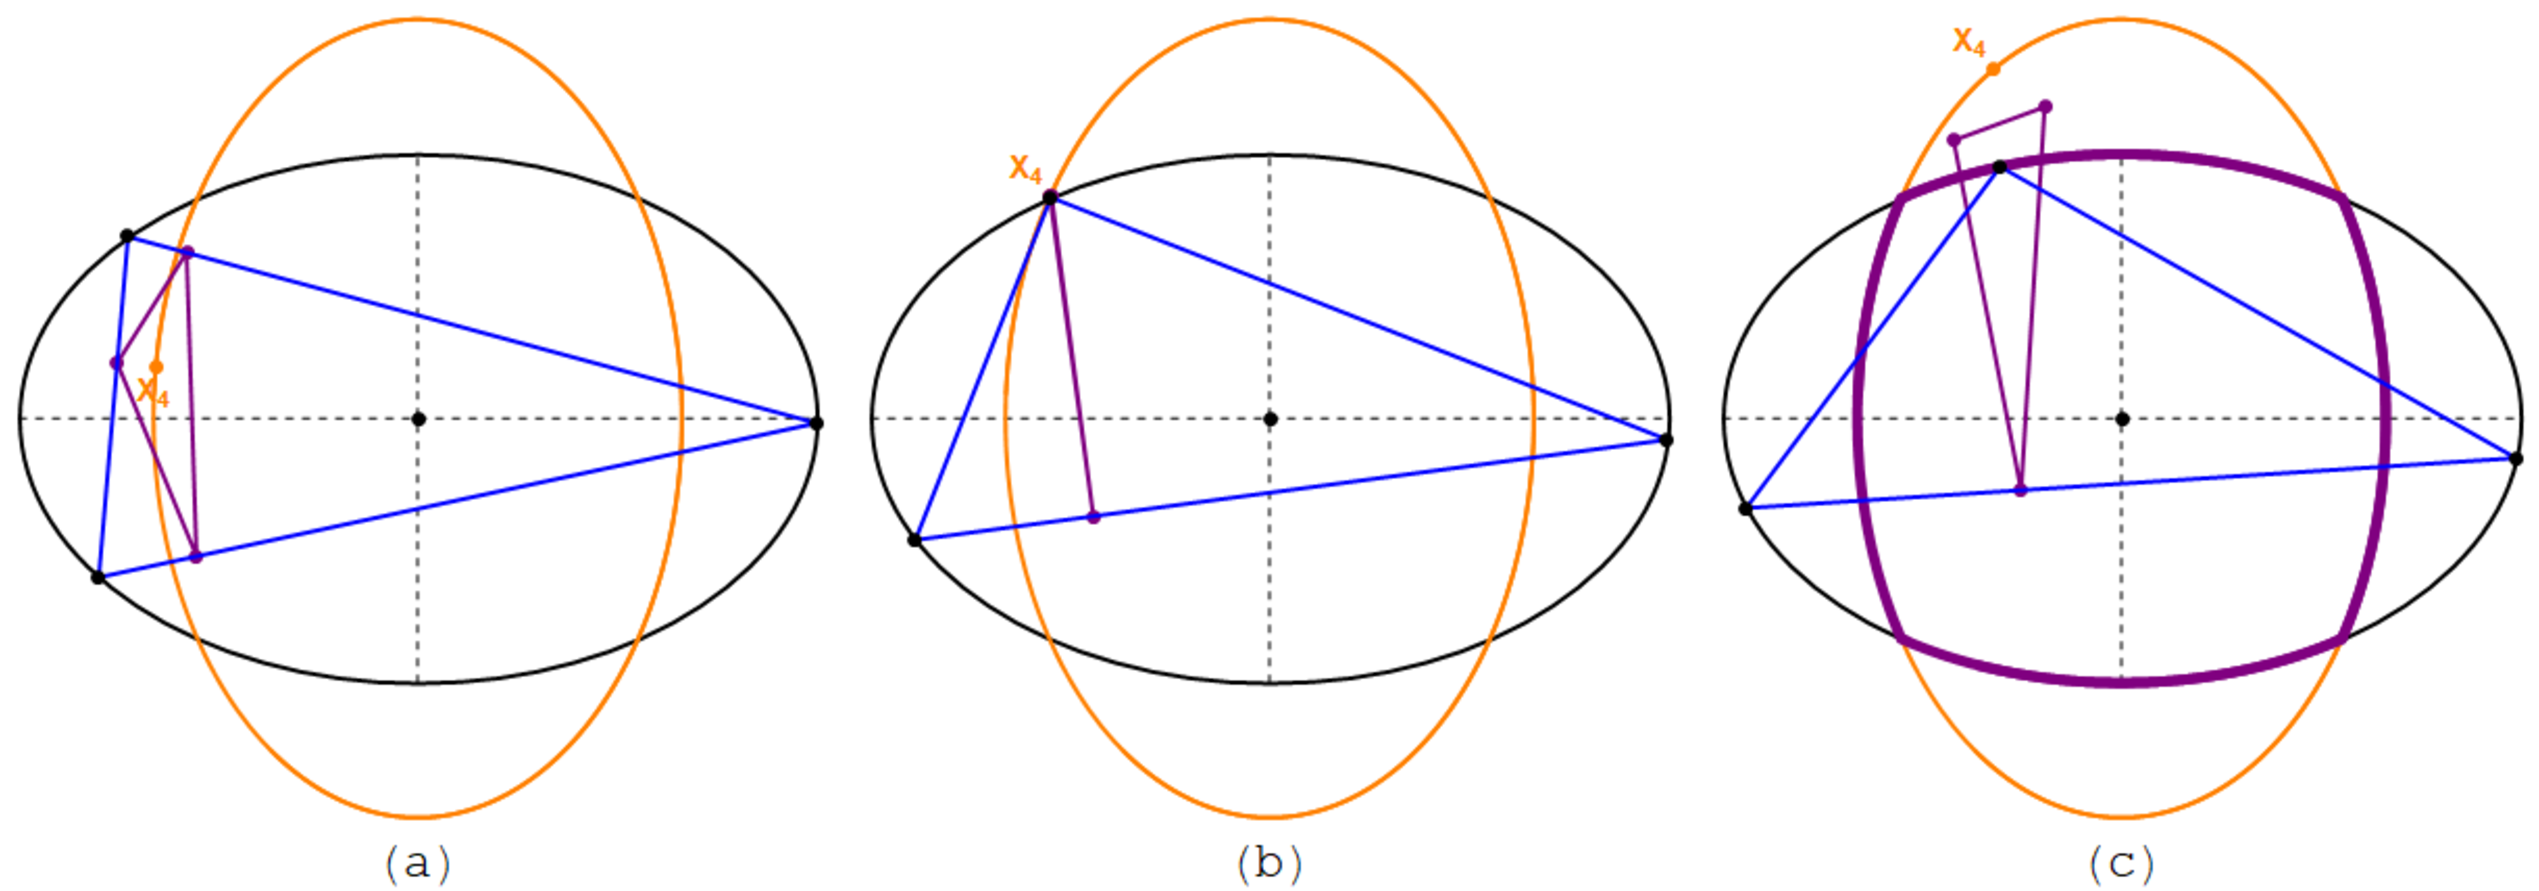
\includegraphics[width=\textwidth]{pics/0045_ort_loci_orthic.pdf}
    \caption{Denote $T$ as an orbit (blue) and $T_h$ its Orthic Triangle (purple). (a) at this orbit position, $X_4$ is inside $B$, $T$ is acute, and $T_h$ is well-conditioned. Its incenter coincides with $X_4$. (b) $X_4$ is now on $B$, $T$ is a right triangle, and $T_h$ degenerates to a segment. (c) $X_4$ lies outside $B$, two of $T_h$'s vertices lie outside $T$. Its incenter separates from $X_4$ and is now congruent with the obtuse vertex. In general, if $a>a_0$, the locus of the Incenter of the Orthic is a four-piecewise-elliptic curve with four kinks.}
    \label{fig:orthic_incenter_locus}
\end{figure}

\begin{observation}
For a Billiard with $a>a_0$ the locus of the Incenter of the orbit's Orthic Triangle is a piecewise-elliptic curve with four kinks.
\end{observation}

\subsection{Complimentary Anticomplementary Phenomena}

Consider the Orbit's Anticomplementary Triangle \cite{mw}, shown in Figure~\ref{fig:act_intouch}. Its own Incircle touches it at three contact points as well as its 9-Point Circle (congruent with the orbit's Circumcircle \cite{mw}) at {\em its} Feuerbach Point. Above it was pointed out the latter's locus is the Billiard. Remarkably:

\begin{observation}
The vertices of the anticomplementary's Intouch Triangle sweep the Billiard.
\end{observation}

\noindent This phenomenon can be viewed here \cite[video \#7]{dsr_main_videos_2019} and proof has been kindly contributed \cite{minevich17,minevich19}.

\begin{figure}[H]
    \centering
    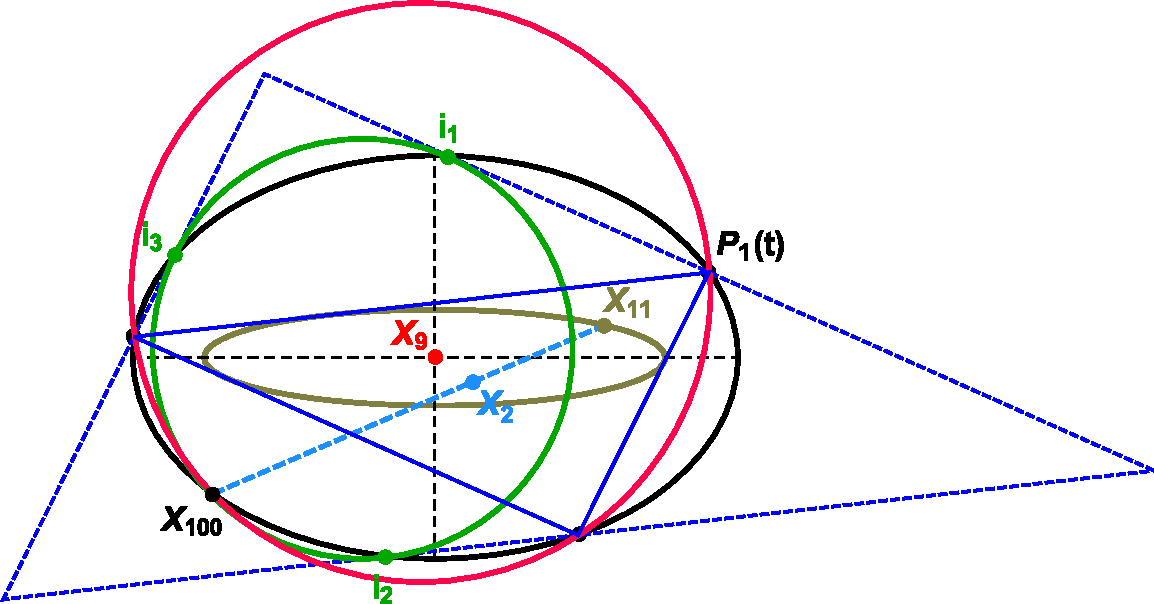
\includegraphics[width=\textwidth]{pics/0048_act_intouch.pdf}
    \caption{The locus of the three Intouch Points $i_1,i_2,i_3$ of the orbit's Anticomplementary Triangle (dashed blue) is the Billiard.}
    \label{fig:act_intouch}
\end{figure}

Furthermore, if $P_1(t)$ moves monotonically in one direction, the Anticomplementary's intouch points will move non-monotonically with respect to $P_1(t)$, Figure~\ref{fig:act-progress}. 

\begin{figure}[H]
    \centering
    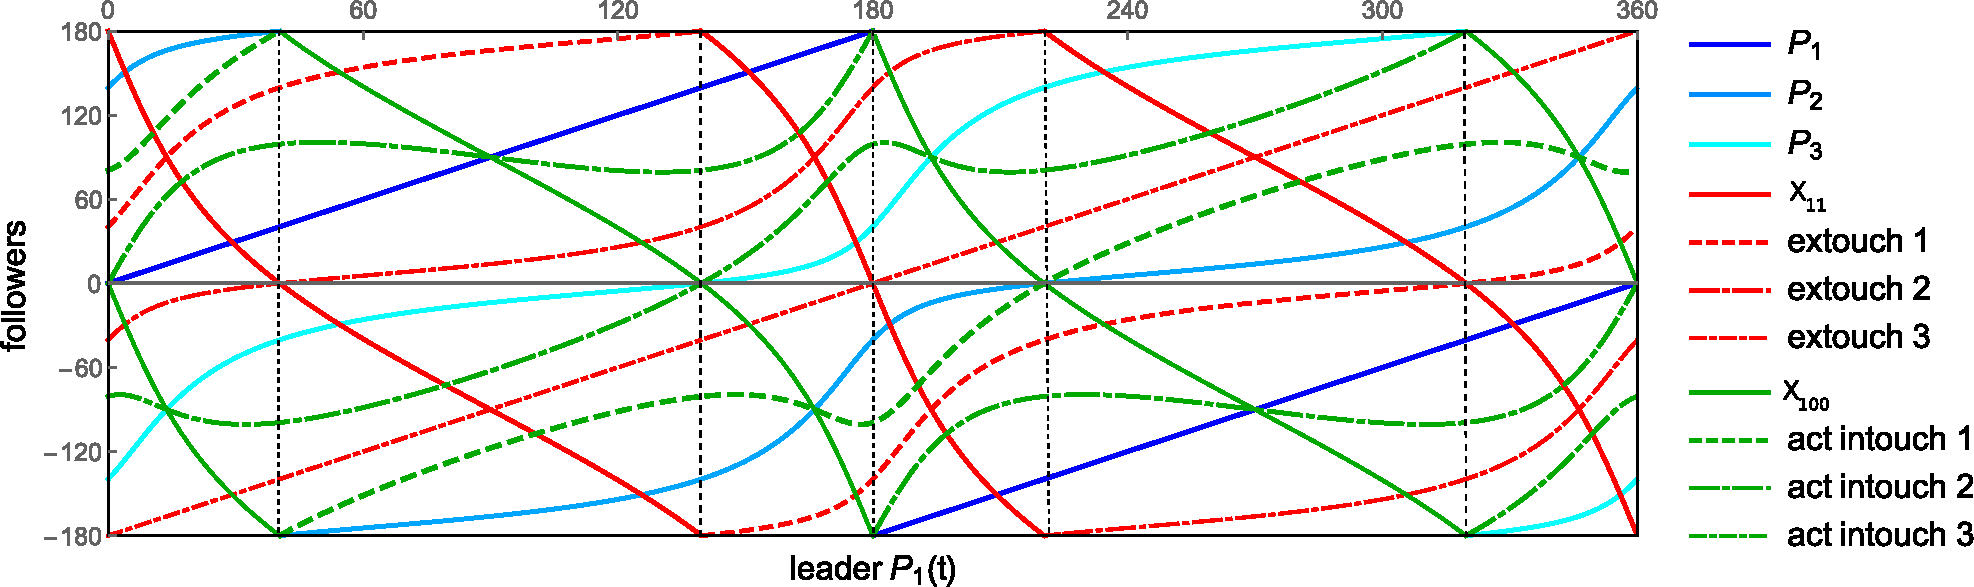
\includegraphics[width=\textwidth]{pics/0049_act_progress.pdf}
    \caption{Angular Progress along the Elliptic Billiard of (i) the $N=3$ orbit vertices $P_1(t)$ (black), $P_2,P_3$ (dark and light blue), (ii) the Feuerbach Point $X_{11}$ (red), always retrograde wrt. $P_1(t)$, (iii) the three Extouch Points (dashed reds) whose direction of motion is the same as $P_1(t)$, (iv) the Feuerbach Point of the Anticomplementary Triangle $X_{100}$ (green), moving opposite to $P_1(t)$, (v) the three Intouch Points of the Anticomplementary Triangle (dashed green), whose angular progress is non-monotonic with respect to $P_1(t)$.}
    \label{fig:act-progress}
\end{figure}


\section{Appendix: Spatial Averages}
\label{sec:space-averages}
We've observed above that the sum of cosines is preserved for the family of orbits as well as the product of cosines for the family of tangential orbits.

Consider more generally, two calculations applicable to all trajectories, closed or not:

\begin{itemize}
    \item $K$ the arithmetic mean of cosines
    \item $K'$ the geometric mean of tangential cosines
\end{itemize}

Parametrize a trajectory family by the minor semiaxis $\beta$ of their confocal caustic, Figure~\ref{fig:gen-caustic-pencil}. Asymptotically:

\begin{eqnarray}
K(\beta)&=&\lim_{M\to\infty}\,\,\frac{1}{M}\,  \sum_{i=1}^{M}{\cos\theta_i}\\
K'(\beta)&=&\lim_{M\to\infty}|\prod_{i=1}^{M}{\cos\theta_i'}|^{1/M}
\end{eqnarray}

Where $\theta_i$ (resp. $\theta_i'$) are the angles between consecutive segments of the trajectory (resp. tangential polygon). For trajectories which do not close, the above will not depend on the starting point on the ellipse (trajectories are space-filling, Figure~\ref{fig:space-filling}). The above expressions become equivalent to the following spatial integrals, whose density depends on $\kappa(s)$, the curvature of the caustic parametrized by arc length \cite{sergei17_curvature}:

\begin{figure}
    \centering
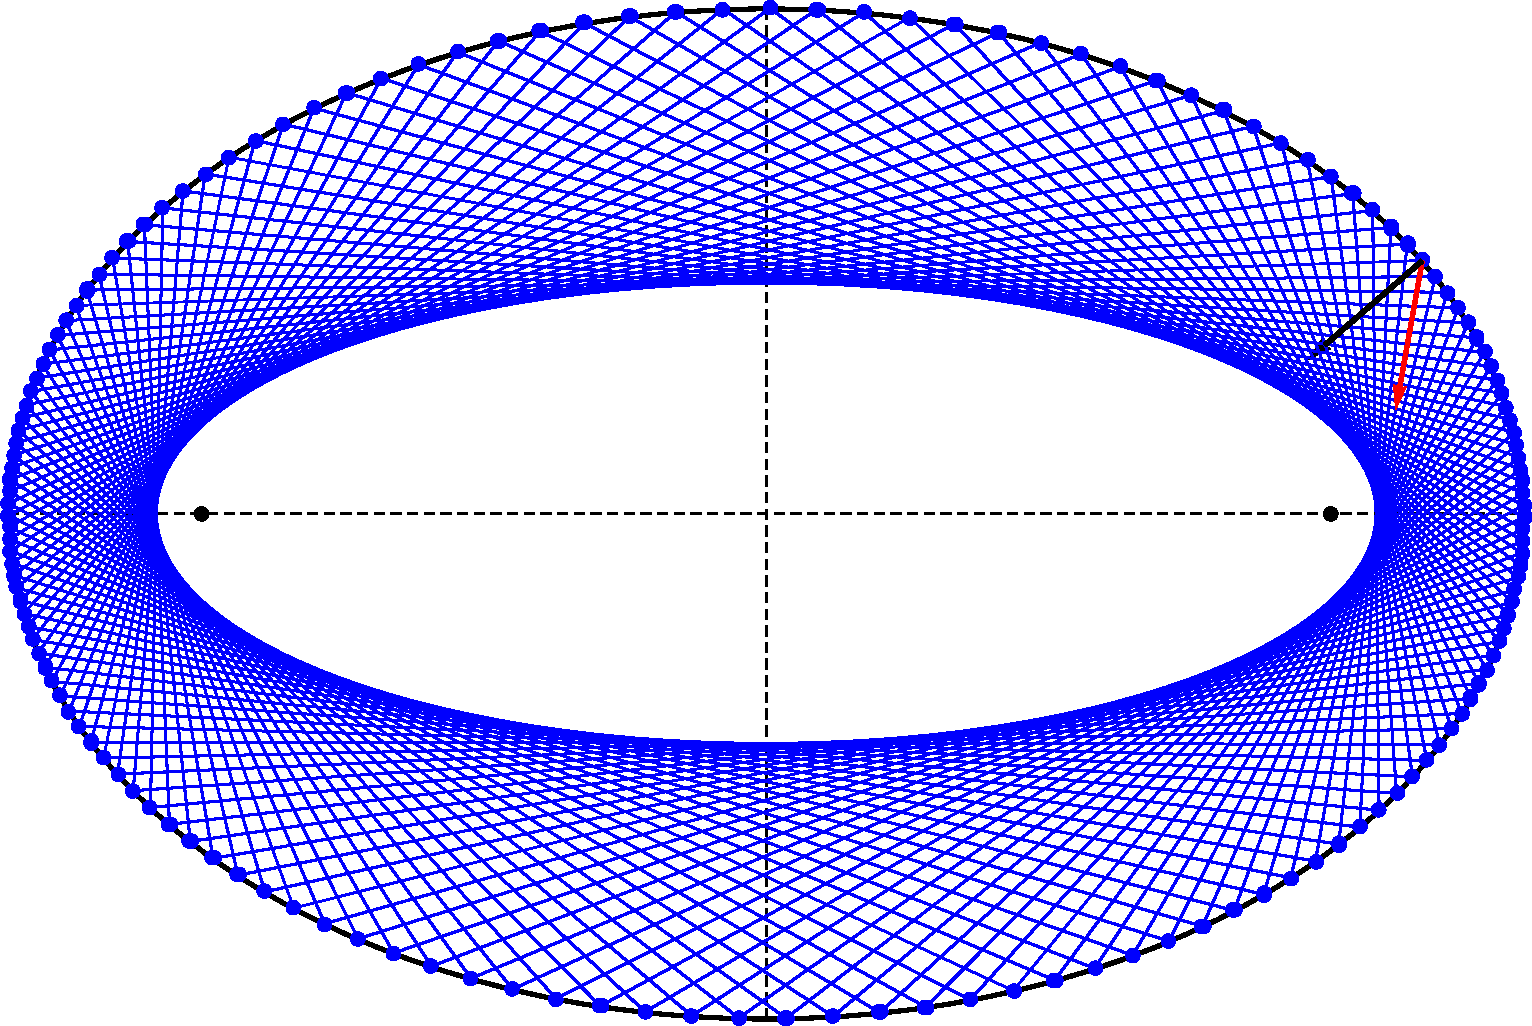
\includegraphics[width=.5\textwidth]{pics/0210_space_filling.pdf}
    \caption{300 edges of a  space-filling trajectory (the starting location and direction is shown by a red arrow on the Billiard's first quadrant.}
    \label{fig:space-filling}
\end{figure}

\begin{eqnarray}
K(\beta)&=&\frac{1}{\Delta}\,\,\oint\,\cos\theta\,\kappa(s)^{2/3}ds\\
\log K'(\beta)&=&\frac{ 1}{\Delta}\,\,\oint \,\log|\cos\theta'|\,\kappa(s)^{2/3}ds\\
\mbox{with}\,\Delta&=&\oint\,\kappa(s)^{2/3}ds
\end{eqnarray}

\begin{figure}
    \centering
    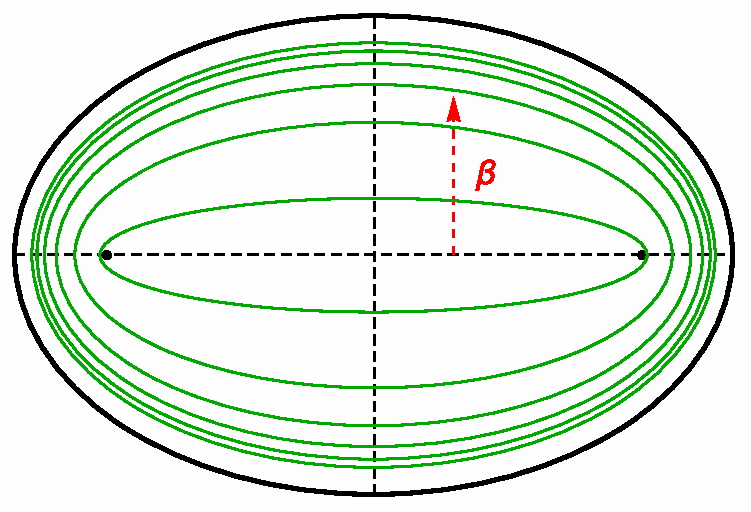
\includegraphics[width=.5\textwidth]{pics/0175_caustic_pencil.pdf}
    \caption{An $a=1.5$ billiard is shown as well as a few members (green) of a continuous pencil of confocal caustics, parametrized by $\beta\in(0,1)$, their minor semiaxis.}
    \label{fig:gen-caustic-pencil}
\end{figure}

These spatial averages  are shown in Figure~\ref{fig:koiller-sum-prod} for $a=5$ (smaller $a$ make the two spatial averages become to close to each other). For values of $\beta$ where the trajectory becomes close, the spatial averages yield numbers which perfectly match mean cosines and geometric mean excentral cosines when these are estimated numerically over an orbit family (not via the integral). It appears that for any $a$, $|K|>K'$.

\begin{figure}
    \centering
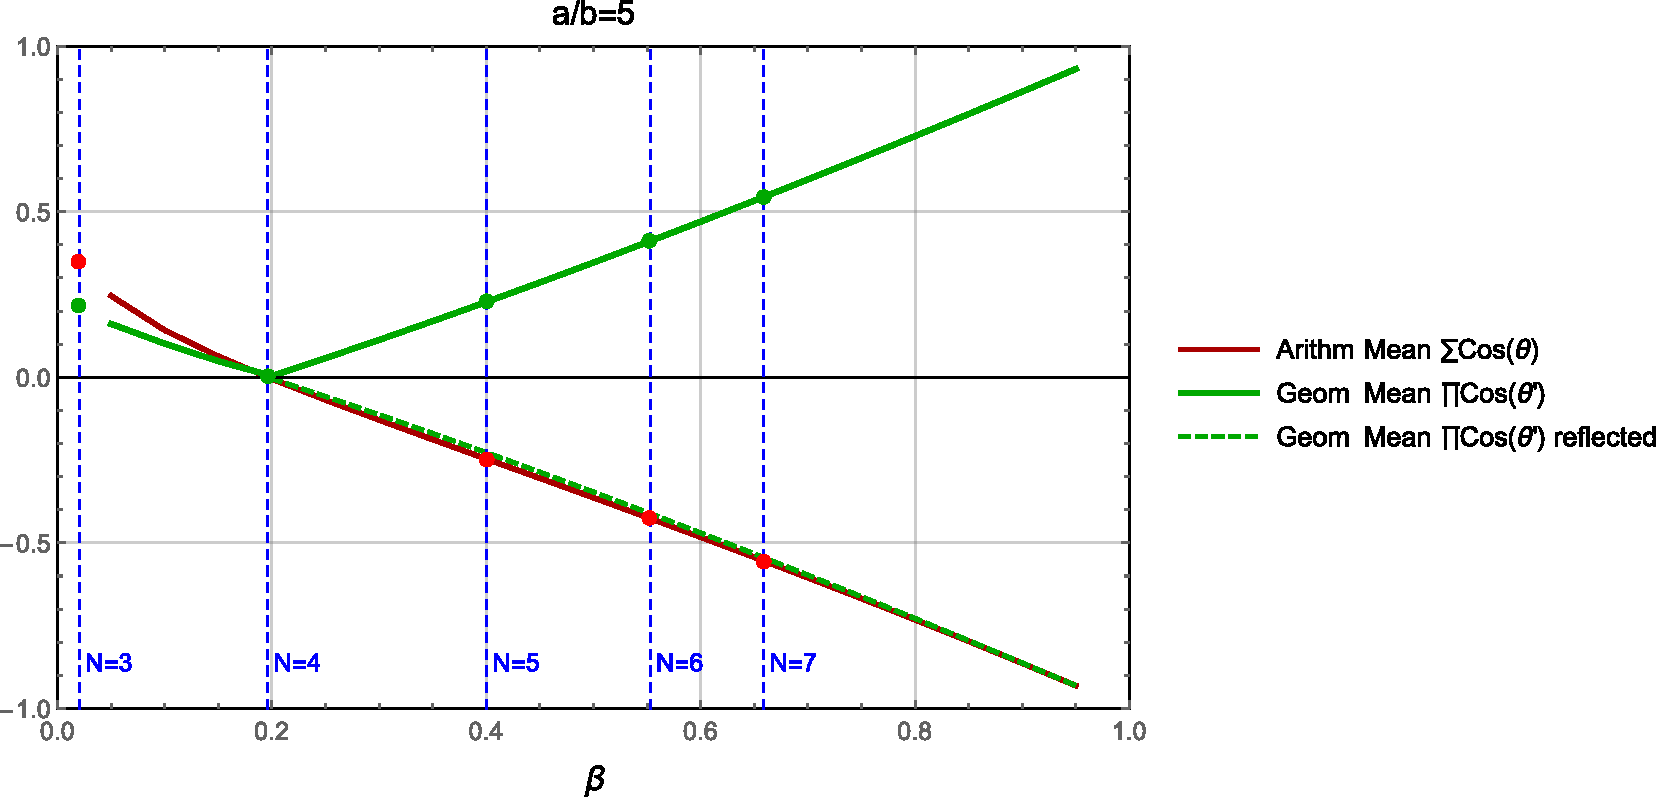
\includegraphics[width=\textwidth]{pics/0172_koiller_sum_prod_a5.pdf}
    \caption{Spatial Averages vs. $\beta$, the caustic minor semiaxis, for $a=5$. Blue dashed vertical lines mark the $\beta$ for non-intersecting orbits. Red: $K$, the arithmetic mean of trajectory cosines. Green: $K'$, the geometric mean of tangential cosines. Dashed green: past the $N=4$ caustic, the $K'$ curve is reflected about the $x$ axis to show it closely tracks $K$ (though they are never the same). Blue and red dots are the same averages obtained via closed-form expressions, perfectly matching the spatial average curves.}
    \label{fig:koiller-sum-prod}
\end{figure}


% BibTeX users please use one of

\bibliographystyle{spmpsci}  % mathematics and 

\bibliography{elliptic_billiards_v2,media}   % name your BibTeX data base

\end{document}
% end of file template.tex